% ===========================================================================
%  SnapCare pill dispenser — assembly guide
%
%  Build:  latexmk -pdf assembly-guide.tex     (or `make guide` one dir up)
%
%  The text follows ../ASSEMBLY.md and the pin map in
%  ../snapcare_dispenser/config.py. If this and config.py ever disagree,
%  config.py is right and this is stale.
% ===========================================================================
\documentclass[11pt,a4paper]{article}
% ---------------------------------------------------------------------------
%  Shared preamble: page setup, palette, boxes, and the icon/figure toolkit.
%  Everything visual in the guide is drawn here or from these styles, so the
%  colour of a wire in one figure is the colour of the same wire everywhere.
% ---------------------------------------------------------------------------
\usepackage[T1]{fontenc}
\usepackage[utf8]{inputenc}
\usepackage{textcomp}
\usepackage{XCharter}
\usepackage[scaled=0.92]{FiraSans}
\usepackage[scaled=0.95]{zi4}
\usepackage{amssymb}
\usepackage[a4paper,top=22mm,bottom=20mm,left=22mm,right=22mm,headsep=7mm]{geometry}
\usepackage{graphicx}
\usepackage{booktabs}
\usepackage{array}
\usepackage{longtable}
\usepackage{multicol}
\usepackage{enumitem}
\usepackage{fancyhdr}
\usepackage{titlesec}
\usepackage{xcolor}
\usepackage{tikz}
\usepackage[most]{tcolorbox}
\usepackage[hidelinks]{hyperref}

\usetikzlibrary{calc,positioning,shapes.geometric,shapes.misc,arrows.meta,
                backgrounds,fit,decorations.pathreplacing,decorations.markings,
                patterns,shadows.blur}

% ── palette ────────────────────────────────────────────────────────────────
% The five signal colours are the ring's own colour vocabulary, taken from
% indicators.py, so a figure of the ring and a figure of a wire agree.
\definecolor{ink}{HTML}{1B1F24}
\definecolor{ink70}{HTML}{4A5057}
\definecolor{ink40}{HTML}{8A9199}
\definecolor{ink15}{HTML}{D8DDE2}
\definecolor{paper}{HTML}{FFFFFF}
\definecolor{shade}{HTML}{F4F6F8}

\definecolor{scred}{HTML}{C2185B}      % accent / raspberry
\definecolor{servo}{HTML}{E8710A}      % servo signal
\definecolor{ringc}{HTML}{9600FF}      % ws2812 data (violet, as the ring)
\definecolor{buzzc}{HTML}{B26A00}      % buzzer
\definecolor{btnc}{HTML}{00857A}       % button
\definecolor{i2cc}{HTML}{005AFF}       % i2c
\definecolor{p33}{HTML}{D24B2E}        % 3V3 rail
\definecolor{p5}{HTML}{B3001B}         % 5V rail
\definecolor{gndc}{HTML}{2B2B2B}       % ground
\definecolor{resv}{HTML}{C9A227}       % reserved, unfitted
\definecolor{avoid}{HTML}{9AA3AB}      % deliberately not used

\definecolor{ledgreen}{HTML}{00C83C}
\definecolor{ledblue}{HTML}{005AFF}
\definecolor{ledamber}{HTML}{FF8200}
\definecolor{ledviolet}{HTML}{9600FF}
\definecolor{ledcyan}{HTML}{00AABE}

\definecolor{okgreen}{HTML}{1E7A3C}
\definecolor{warnamber}{HTML}{9A6400}
\definecolor{dangerred}{HTML}{B3001B}

% ── shorthands for the units this guide keeps repeating ────────────────────
\newcommand{\ohm}{\,\textohm}
\newcommand{\uF}{\,\textmu F}
\newcommand{\dgr}{\textdegree}
\newcommand{\iic}{I\textsuperscript{2}C}
\newcommand{\gpio}[1]{\mbox{GPIO~#1}}
\newcommand{\pin}[1]{\mbox{pin~#1}}
\newcommand{\code}[1]{\texttt{#1}}

% ── headings ───────────────────────────────────────────────────────────────
\titleformat{\section}
  {\sffamily\bfseries\Large\color{ink}}{\thesection}{0.6em}{}
  [\vspace{-0.6ex}{\color{ink15}\titlerule[1.1pt]}]
\titleformat{\subsection}
  {\sffamily\bfseries\large\color{ink}}{\thesubsection}{0.5em}{}
\titlespacing*{\section}{0pt}{2.2ex plus 1ex minus .2ex}{1.4ex plus .2ex}
\titlespacing*{\subsection}{0pt}{1.8ex plus 1ex minus .2ex}{0.9ex plus .2ex}

\setlength{\headheight}{14pt}
\pagestyle{fancy}
\fancyhf{}
\renewcommand{\headrulewidth}{0.4pt}
\renewcommand{\headrule}{\hbox to\headwidth{\color{ink15}\leaders\hrule height \headrulewidth\hfill}}
\fancyhead[L]{\sffamily\small\color{ink40}SnapCare pill dispenser \textendash{} assembly}
\fancyhead[R]{\sffamily\small\color{ink40}\leftmark}
\fancyfoot[C]{\sffamily\small\color{ink40}\thepage}

% ── code listings ──────────────────────────────────────────────────────────
\tcbuselibrary{listings,breakable,skins}
\lstdefinestyle{shellstyle}{
  basicstyle=\ttfamily\footnotesize\color{ink},
  breaklines=true, breakatwhitespace=false,
  columns=fullflexible, keepspaces=true,
  showstringspaces=false,
  commentstyle=\color{ink40}\itshape,
  morecomment=[l]{\#},
}
\newtcblisting{shell}{
  listing only, listing style=shellstyle,
  colback=shade, colframe=ink15, boxrule=0.6pt, arc=2pt,
  left=2mm, right=2mm, top=1.4mm, bottom=1.4mm,
  before skip=1.6ex, after skip=1.6ex,
}
\newtcblisting{pycode}{
  listing only,
  listing style=shellstyle,
  colback=shade, colframe=ink15, boxrule=0.6pt, arc=2pt,
  left=2mm, right=2mm, top=1.4mm, bottom=1.4mm,
  before skip=1.6ex, after skip=1.6ex,
}

% ── callout boxes ──────────────────────────────────────────────────────────
\newtcolorbox{provebox}[1][]{
  enhanced, breakable,
  colback=white, colframe=okgreen, boxrule=0pt,
  leftrule=2.4pt, arc=0pt, outer arc=0pt,
  left=3.5mm, right=3mm, top=2mm, bottom=2mm,
  borderline west={2.4pt}{0pt}{okgreen},
  title=\relax, #1
}
\newtcolorbox{warnbox}[1][]{
  enhanced, breakable,
  colback=warnamber!5, colframe=warnamber!45, boxrule=0.7pt, arc=2pt,
  left=3mm, right=3mm, top=2mm, bottom=2mm, #1
}
\newtcolorbox{dangerbox}[1][]{
  enhanced, breakable,
  colback=dangerred!5, colframe=dangerred!55, boxrule=0.9pt, arc=2pt,
  left=3mm, right=3mm, top=2mm, bottom=2mm, #1
}
\newtcolorbox{notebox}[1][]{
  enhanced, breakable,
  colback=shade, colframe=ink15, boxrule=0.7pt, arc=2pt,
  left=3mm, right=3mm, top=2mm, bottom=2mm, #1
}

\newcommand{\provetitle}{\textbf{\sffamily\color{okgreen}Prove it}\par\vspace{0.6ex}}
\newcommand{\warntitle}[1]{\textbf{\sffamily\color{warnamber}#1}\par\vspace{0.6ex}}
\newcommand{\dangertitle}[1]{\textbf{\sffamily\color{dangerred}#1}\par\vspace{0.6ex}}

% Caption styling
\usepackage[font={small,sf},labelfont={bf,color=ink70},textfont={color=ink70}]{caption}

% ── table helpers ──────────────────────────────────────────────────────────
\renewcommand{\arraystretch}{1.25}
\newcommand{\hdr}[1]{\textbf{\sffamily\small #1}}
\newcommand{\chk}{$\square$~}

% Colour swatch used in wire tables: a short length of the wire's own colour.
\newcommand{\swatch}[1]{\tikz[baseline=-0.5ex]{\draw[#1,line width=2.4pt,line cap=round] (0,0)--(0.5,0);}}

% ═══════════════════════════════════════════════════════════════════════════
%  ICONS  —  small line drawings for the bill of materials
% ═══════════════════════════════════════════════════════════════════════════
\tikzset{
  icn/.style={line width=0.7pt, color=ink70},
  icnfill/.style={fill=ink15},
}
% Each icon draws into a 12mm x 9mm box so the BOM column stays even.
\newcommand{\iconbox}[1]{%
  \begin{tikzpicture}[scale=1,every node/.style={font=\tiny\sffamily}]
    \path (-0.6,-0.45) rectangle (0.6,0.45);
    #1
  \end{tikzpicture}%
}

\newcommand{\iconpi}{\iconbox{%
  \draw[icn,fill=okgreen!12,rounded corners=1pt] (-0.55,-0.34) rectangle (0.55,0.34);
  \foreach \x in {-0.45,-0.37,...,0.35}{
    \fill[ink70] (\x,0.24) circle (0.022);
    \fill[ink70] (\x,0.15) circle (0.022);}
  \draw[icn,fill=ink15] (-0.42,-0.26) rectangle (-0.02,-0.02);
  \draw[icn] (0.12,-0.26) rectangle (0.5,-0.06);
}}

\newcommand{\iconsd}{\iconbox{%
  \draw[icn,fill=ink15] (-0.28,-0.36) -- (0.3,-0.36) -- (0.3,0.24) -- (0.16,0.38)
        -- (-0.28,0.38) -- cycle;
  \foreach \x in {-0.16,-0.06,0.04,0.14}{\draw[icn] (\x,0.34) -- (\x,0.18);}
}}

\newcommand{\iconpsu}{\iconbox{%
  \draw[icn,fill=ink15,rounded corners=1pt] (-0.55,-0.26) rectangle (0.1,0.26);
  \node[color=ink70,font=\tiny\sffamily\bfseries] at (-0.22,0) {5V};
  \draw[icn] (0.1,0.12) -- (0.34,0.12); \draw[icn] (0.1,-0.12) -- (0.34,-0.12);
  \draw[icn,fill=white] (0.34,0.04) rectangle (0.5,0.2);
  \draw[icn,fill=white] (0.34,-0.2) rectangle (0.5,-0.04);
}}

\newcommand{\iconservo}{\iconbox{%
  \draw[icn,fill=ink15] (-0.34,-0.3) rectangle (0.16,0.24);
  \draw[icn,fill=white] (-0.46,0.02) rectangle (0.28,0.14);
  \draw[icn,fill=servo!25] (0.16,-0.06) circle (0.13);
  \draw[icn,line width=1pt,servo] (0.16,-0.06) -- (0.5,-0.3);
  \draw[icn] (-0.34,-0.3) -- (-0.5,-0.42);
}}

\newcommand{\iconring}{\iconbox{%
  \draw[icn] (0,0) circle (0.32);
  \draw[icn] (0,0) circle (0.17);
  \foreach \a in {0,30,...,330}{
    \fill[ringc!70] (\a:0.245) circle (0.035);}
}}

\newcommand{\iconbuzzer}{\iconbox{%
  \draw[icn,fill=ink15] (-0.1,0) circle (0.26);
  \draw[icn,fill=ink40] (-0.1,0) circle (0.08);
  \foreach \r in {0.34,0.44}{
    \draw[icn,buzzc] (0.02,0) ++(-55:\r) arc (-55:55:\r);}
}}

\newcommand{\iconbutton}{\iconbox{%
  \draw[icn,fill=ink15] (-0.3,-0.3) rectangle (0.3,0.0);
  \draw[icn,fill=btnc!30] (0,0.0) ellipse (0.16 and 0.07);
  \draw[icn] (-0.16,0.0) -- (-0.16,0.14) arc (180:0:0.16 and 0.1) -- (0.16,0.0);
  \draw[icn] (-0.22,-0.3) -- (-0.22,-0.42);
  \draw[icn] (0.22,-0.3) -- (0.22,-0.42);
}}

\newcommand{\iconrtc}{\iconbox{%
  \draw[icn,fill=i2cc!8] (-0.5,-0.3) rectangle (0.5,0.3);
  \draw[icn,fill=ink15] (0.06,-0.02) circle (0.2);
  \node[color=ink40,font=\tiny\sffamily] at (0.06,-0.02) {\tiny +};
  \draw[icn,fill=ink40] (-0.42,-0.16) rectangle (-0.2,0.16);
  \foreach \y in {-0.24,-0.12,0.0,0.12}{\fill[ink70] (0.44,\y) circle (0.025);}
}}

\newcommand{\iconcap}{\iconbox{%
  \draw[icn,fill=ink15,rounded corners=1pt] (-0.16,-0.28) rectangle (0.16,0.28);
  \draw[icn,fill=ink40] (-0.16,-0.28) rectangle (-0.05,0.28);
  \draw[icn] (-0.06,-0.28) -- (-0.06,-0.44);
  \draw[icn] (0.08,-0.28) -- (0.08,-0.44);
  \node[color=ink70,font=\tiny\sffamily] at (0.32,0.1) {--};
}}

\newcommand{\iconres}{\iconbox{%
  \draw[icn] (-0.5,0) -- (-0.28,0);
  \draw[icn] (-0.28,0) -- (-0.22,0.16) -- (-0.1,-0.16) -- (0.02,0.16)
            -- (0.14,-0.16) -- (0.22,0) -- (0.5,0);
}}

\newcommand{\iconwire}{\iconbox{%
  \draw[icn,servo,line width=1pt] (-0.5,-0.2) .. controls (-0.1,0.36) and (0.1,-0.36) .. (0.5,0.2);
  \draw[icn,fill=ink15] (-0.5,-0.28) rectangle (-0.4,-0.12);
  \draw[icn,fill=ink15] (0.4,0.12) rectangle (0.5,0.28);
}}

\newcommand{\iconcloud}{\iconbox{%
  \draw[icn,fill=ink15] (-0.3,-0.1) arc (180:360:0.3 and 0.22)
        -- (0.3,-0.1) arc (-20:200:0.32 and 0.24) -- cycle;
  \draw[icn] (0,-0.14) -- (0,-0.34);
  \draw[icn] (-0.12,-0.34) -- (0.12,-0.34);
}}

% ═══════════════════════════════════════════════════════════════════════════
%  THE 40-PIN HEADER
% ═══════════════════════════════════════════════════════════════════════════
% One macro, one data table. Every stage figure that shows a pin takes its
% colour from the same style list, so a pin is the same colour wherever it
% appears in the guide.
\tikzset{
  padbase/.style={rounded corners=1pt, draw=ink40, line width=0.5pt,
                  minimum width=6.4mm, minimum height=3.9mm, inner sep=0pt,
                  font=\sffamily\scriptsize},
  pfree/.style={padbase, fill=white, text=ink40},
  pavoid/.style={padbase, fill=avoid!18, text=ink40, draw=avoid},
  pgnd/.style={padbase, fill=gndc!85, text=white, draw=gndc},
  ppwr33/.style={padbase, fill=p33!18, text=p33!80!black, draw=p33!60},
  ppwr5/.style={padbase, fill=p5!14, text=p5!80!black, draw=p5!55},
  puse33/.style={padbase, fill=p33, text=white, draw=p33!70!black, line width=0.9pt},
  pusei2c/.style={padbase, fill=i2cc, text=white, draw=i2cc!70!black, line width=0.9pt},
  puseservo/.style={padbase, fill=servo, text=white, draw=servo!70!black, line width=0.9pt},
  pusering/.style={padbase, fill=ringc, text=white, draw=ringc!70!black, line width=0.9pt},
  pusebuzz/.style={padbase, fill=buzzc, text=white, draw=buzzc!70!black, line width=0.9pt},
  pusebtn/.style={padbase, fill=btnc, text=white, draw=btnc!70!black, line width=0.9pt},
  pusegnd/.style={padbase, fill=gndc, text=white, draw=gndc, line width=0.9pt},
  presv/.style={padbase, fill=resv!22, text=resv!45!black, draw=resv!70, dashed},
  plabel/.style={font=\sffamily\scriptsize, text=ink70, inner sep=1pt},
  plabelon/.style={font=\sffamily\scriptsize\bfseries, text=ink, inner sep=1pt},
}

% \headerfigure{row spacing}  — draws the whole 40-pin header, top to bottom.
\newcommand{\drawheader}[1][0.62]{%
  \def\rowsep{#1}
  % board outline behind the pins
  \begin{scope}[on background layer]
    \fill[shade, rounded corners=2pt]
      (-4.9,0.62) rectangle (4.9,{-\rowsep*20-0.28});
  \end{scope}
  \node[font=\sffamily\bfseries\small, text=ink] at (0,0.36)
    {Raspberry Pi 3B \textendash{} 40-pin header};
  \node[font=\sffamily\scriptsize, text=ink70] at (0,0.06)
    {pin 1 is the corner nearest the microSD / power end};
  \foreach \r/\lb/\ls/\rb/\rs in {%
      1/{3V3}/{puse33}/{5V}/{ppwr5},
      2/{GPIO2 SDA}/{pusei2c}/{5V}/{ppwr5},
      3/{GPIO3 SCL}/{pusei2c}/{GND}/{pusegnd},
      4/{GPIO4}/{pfree}/{GPIO14 TXD}/{pavoid},
      5/{GND}/{pfree}/{GPIO15 RXD}/{pavoid},
      6/{GPIO17}/{puseservo}/{GPIO18}/{pusering},
      7/{GPIO27}/{puseservo}/{GND}/{pusegnd},
      8/{GPIO22}/{puseservo}/{GPIO23}/{pusebuzz},
      9/{3V3}/{ppwr33}/{GPIO24}/{pusebtn},
      10/{GPIO10}/{pavoid}/{GND}/{pusegnd},
      11/{GPIO9}/{pavoid}/{GPIO25}/{pfree},
      12/{GPIO11}/{pavoid}/{GPIO8}/{pavoid},
      13/{GND}/{pfree}/{GPIO7}/{pavoid},
      14/{GPIO0 ID}/{pavoid}/{GPIO1 ID}/{pavoid},
      15/{GPIO5}/{presv}/{GND}/{pfree},
      16/{GPIO6}/{presv}/{GPIO12}/{pfree},
      17/{GPIO13}/{presv}/{GND}/{pfree},
      18/{GPIO19}/{presv}/{GPIO16}/{pfree},
      19/{GPIO26}/{presv}/{GPIO20}/{pfree},
      20/{GND}/{pfree}/{GPIO21}/{pfree}%
    }{%
    \pgfmathtruncatemacro{\lp}{2*\r-1}%
    \pgfmathtruncatemacro{\rp}{2*\r}%
    \pgfmathsetmacro{\yy}{-\rowsep*\r}%
    \node[\ls] (L\lp) at (-0.62,\yy) {\lp};
    \node[\rs] (R\rp) at (0.62,\yy) {\rp};
    \node[plabel, anchor=east] at (-1.05,\yy) {\lb};
    \node[plabel, anchor=west] at (1.05,\yy) {\rb};
  }%
}

% A compact legend for the header figure.
\newcommand{\headerlegend}{%
  \begin{tikzpicture}[every node/.style={font=\sffamily\scriptsize,text=ink70}]
    \def\sw##1##2##3{\node[##1,minimum width=4.6mm,minimum height=3.2mm] at (##2,0) {};
                     \node[anchor=west] at (##2+0.28,0) {##3};}
    \sw{puseservo}{0}{servo signal}
    \sw{pusering}{2.9}{ring data}
    \sw{pusebuzz}{5.3}{buzzer}
    \sw{pusebtn}{7.3}{button}
    \sw{pusei2c}{9.1}{\iic{} (RTC)}
    \begin{scope}[yshift=-0.52cm]
      \sw{puse33}{0}{3V3 to RTC}
      \sw{pusegnd}{2.9}{ground, used}
      \sw{presv}{5.3}{reserved, trays 4--8}
      \sw{pavoid}{8.6}{deliberately avoided}
    \end{scope}
  \end{tikzpicture}%
}

% ═══════════════════════════════════════════════════════════════════════════
%  WIRING-FIGURE TOOLKIT  —  used by every stage
% ═══════════════════════════════════════════════════════════════════════════
\tikzset{
  modbox/.style={draw=ink70, line width=0.8pt, fill=white, rounded corners=2pt,
                 minimum width=30mm, minimum height=14mm, align=center,
                 font=\sffamily\small},
  modtitle/.style={font=\sffamily\bfseries\small, text=ink},
  term/.style={circle, draw=ink70, fill=white, line width=0.5pt,
               inner sep=0.6pt, minimum size=2.6mm, font=\sffamily\tiny},
  wire/.style={line width=1.5pt, line cap=round, rounded corners=2pt},
  wlabel/.style={font=\sffamily\scriptsize, text=ink70, fill=white,
                 inner sep=1pt, midway},
  hnote/.style={font=\sffamily\scriptsize\itshape, text=ink40},
  compbox/.style={draw=ink40, line width=0.6pt, fill=shade, rounded corners=1.5pt,
                  font=\sffamily\scriptsize, inner sep=2.4pt, align=center},
}

% A short vertical strip of header pins, for stage figures: only the pins that
% matter, in their real order, with a break marker where pins are skipped.
% \pinstrip{x}{y}{list of pin/label/style}
\newcommand{\pinstriptitle}[2]{%
  \node[font=\sffamily\bfseries\scriptsize,text=ink] at (#1,#2) {Pi header};}

\renewcommand{\sectionmark}[1]{\markboth{#1}{#1}}

% A single header pad in a stage figure. Named H<pin>, so wires can say (H11).
% #1 x  #2 y  #3 physical pin  #4 pad style  #5 label, placed to the right
\newcommand{\hpin}[5]{%
  \node[#4] (H#3) at (#1,#2) {#3};
  \node[plabel, anchor=west] at ({#1+0.42},#2) {#5};
}
% The "some pins are skipped here" marker.
\newcommand{\hgap}[2]{\node[font=\scriptsize, text=ink40] at (#1,#2) {$\vdots$};}
% A frame with a caption behind a strip of pads.
\newcommand{\hframe}[4]{% #1 x #2 ytop #3 ybottom #4 caption
  \begin{scope}[on background layer]
    \fill[shade, rounded corners=2pt]
      ({#1-0.55},{#2+0.34}) rectangle ({#1+2.5},{#3-0.28});
  \end{scope}
  \node[font=\sffamily\scriptsize\bfseries, text=ink40, anchor=west]
       at ({#1-0.5},{#2+0.62}) {#4};
}

% A fake QR code: deterministic, decorative, obviously not scannable at this size.
\newcommand{\fakeqr}[2]{% #1 size in cm, #2 seed integer
  \begin{scope}
    \pgfmathsetmacro{\cell}{#1/11}
    \fill[white] (0,0) rectangle (#1,#1);
    \foreach \i in {0,...,10}{\foreach \j in {0,...,10}{
      \pgfmathtruncatemacro{\bit}{mod(\i*\i*3 + \j*5 + \i*\j*#2 + #2, 7)}
      \ifnum\bit<3
        \fill[ink] ({\i*\cell},{\j*\cell}) rectangle ({(\i+1)*\cell},{(\j+1)*\cell});
      \fi}}
    % three finder patterns
    \foreach \fx/\fy in {0/8,0/0,8/0}{
      \fill[white] ({\fx*\cell-0.02},{\fy*\cell-0.02})
                   rectangle ({(\fx+3)*\cell+0.02},{(\fy+3)*\cell+0.02});
      \fill[ink]   ({\fx*\cell},{\fy*\cell}) rectangle ({(\fx+3)*\cell},{(\fy+3)*\cell});
      \fill[white] ({(\fx+0.55)*\cell},{(\fy+0.55)*\cell})
                   rectangle ({(\fx+2.45)*\cell},{(\fy+2.45)*\cell});
      \fill[ink]   ({(\fx+1)*\cell},{(\fy+1)*\cell})
                   rectangle ({(\fx+2)*\cell},{(\fy+2)*\cell});}
  \end{scope}
}

% resistor drawn inline on a wire between two coordinates
\newcommand{\inlineres}[4]{% #1 colour #2 from #3 to #4 label
  \coordinate (rA) at ($(#2)!0.38!(#3)$);
  \coordinate (rB) at ($(#2)!0.62!(#3)$);
  \draw[wire,#1] (#2) -- (rA);
  \draw[wire,#1] (rB) -- (#3);
  \draw[ink70,line width=0.7pt,fill=white] ($(rA)!0.5!(rB)$) ellipse (0.34 and 0.13);
  \node[font=\sffamily\tiny,text=ink] at ($(rA)!0.5!(rB)$) {#4};
}


\hypersetup{
  pdftitle={SnapCare pill dispenser — assembly guide},
  pdfsubject={Raspberry Pi 3B build, stage by stage},
  pdfauthor={Team H1 — SnapCare},
}

\begin{document}

% ═══════════════════════════════════════════════════════════════════════════
%  COVER
% ═══════════════════════════════════════════════════════════════════════════
\thispagestyle{empty}
\begin{center}
\vspace*{12mm}

{\sffamily\bfseries\fontsize{30}{34}\selectfont\color{ink}
 Building the dispenser}

\vspace{2.5mm}
{\sffamily\large\color{ink70}
 A bare Raspberry Pi 3B to a machine that drops a pill and chirps about it}

\vspace{1.5mm}
{\sffamily\small\color{ink40}
 SnapCare \textperiodcentered{} Team H1 \textperiodcentered{} 16th e-ICON World Contest}

\vfill

% ── hero figure: the whole machine on one page ────────────────────────────
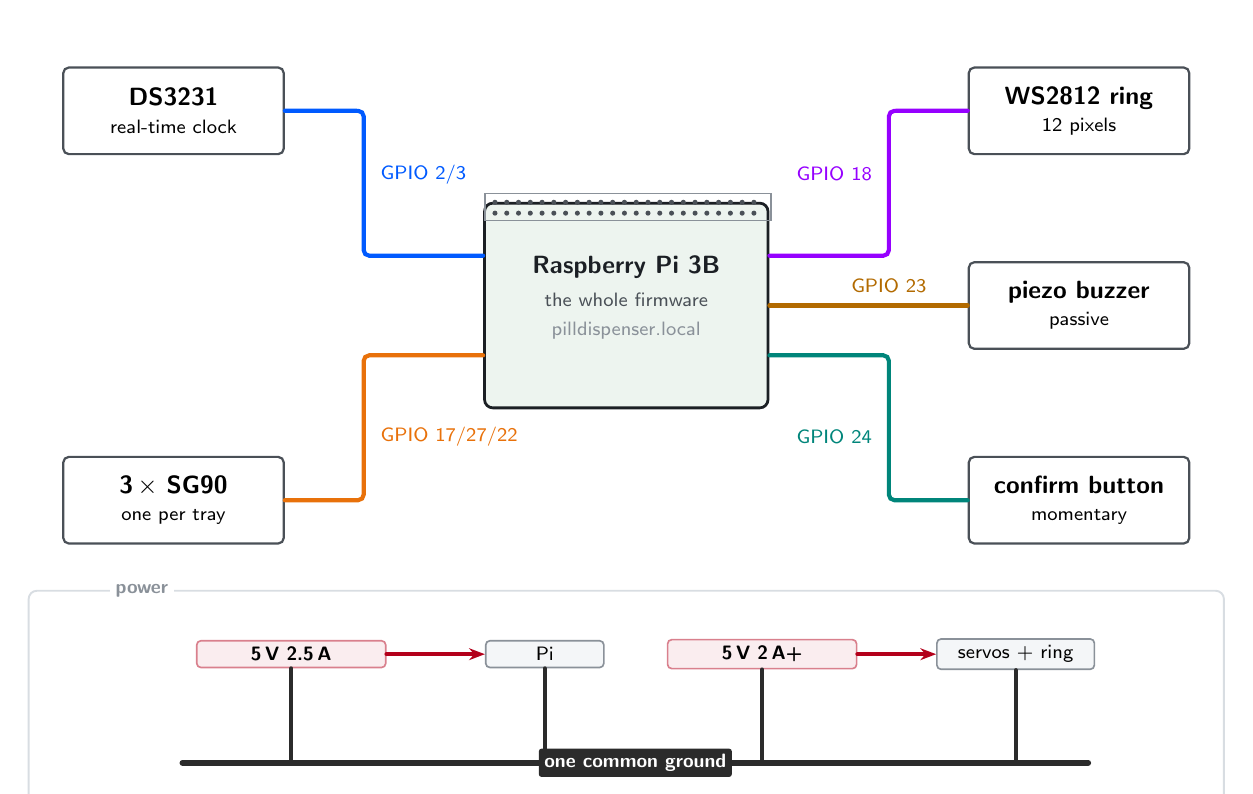
\begin{tikzpicture}[scale=1.15]

  % --- the Pi ---
  \node[draw=ink, line width=1pt, fill=okgreen!8, rounded corners=3pt,
        minimum width=36mm, minimum height=26mm, align=center] (pi) at (0,0) {};
  \node[modtitle] at (0,0.42) {Raspberry Pi 3B};
  \node[font=\sffamily\scriptsize, text=ink70] at (0,0.06) {the whole firmware};
  \node[font=\sffamily\scriptsize, text=ink40] at (0,-0.28) {pilldispenser.local};
  % header pins along the top of the board
  \foreach \x in {-1.45,-1.32,...,1.5}{
    \fill[ink70] (\x,1.14) circle (0.028);
    \fill[ink70] (\x,1.02) circle (0.028);}
  \draw[ink40, line width=0.5pt] (-1.56,0.94) rectangle (1.6,1.24);

  % --- peripherals: two columns, generous vertical spacing ---
  \node[modbox, minimum width=28mm, minimum height=11mm] (rtc) at (-5.0,2.15)
       {\textbf{DS3231}\\[-0.3ex]{\scriptsize real-time clock}};
  \node[modbox, minimum width=28mm, minimum height=11mm] (srv) at (-5.0,-2.15)
       {\textbf{3\,$\times$ SG90}\\[-0.3ex]{\scriptsize one per tray}};
  \node[modbox, minimum width=28mm, minimum height=11mm] (ring) at (5.0,2.15)
       {\textbf{WS2812 ring}\\[-0.3ex]{\scriptsize 12 pixels}};
  \node[modbox, minimum width=28mm, minimum height=11mm] (buz) at (5.0,0)
       {\textbf{piezo buzzer}\\[-0.3ex]{\scriptsize passive}};
  \node[modbox, minimum width=28mm, minimum height=11mm] (btn) at (5.0,-2.15)
       {\textbf{confirm button}\\[-0.3ex]{\scriptsize momentary}};

  % --- signal wires, orthogonal, labels on the vertical legs ---
  \draw[wire, i2cc]  (pi.west|-0,0.55) -- (-2.9,0.55) -- (-2.9,2.15) -- (rtc.east);
  \node[font=\sffamily\scriptsize, text=i2cc, anchor=west] at (-2.82,1.45) {GPIO 2/3};

  \draw[wire, servo] (pi.west|-0,-0.55) -- (-2.9,-0.55) -- (-2.9,-2.15) -- (srv.east);
  \node[font=\sffamily\scriptsize, text=servo, anchor=west] at (-2.82,-1.45) {GPIO 17/27/22};

  \draw[wire, ringc] (pi.east|-0,0.55) -- (2.9,0.55) -- (2.9,2.15) -- (ring.west);
  \node[font=\sffamily\scriptsize, text=ringc, anchor=east] at (2.82,1.45) {GPIO 18};

  \draw[wire, buzzc] (pi.east) -- (buz.west);
  \node[font=\sffamily\scriptsize, text=buzzc, above] at (2.9,0.04) {GPIO 23};

  \draw[wire, btnc]  (pi.east|-0,-0.55) -- (2.9,-0.55) -- (2.9,-2.15) -- (btn.west);
  \node[font=\sffamily\scriptsize, text=btnc, anchor=east] at (2.82,-1.45) {GPIO 24};

  % --- power, as its own band so no supply wire crosses a signal wire ---
  \draw[ink15, line width=0.7pt, rounded corners=3pt] (-6.6,-5.5) rectangle (6.6,-3.15);
  \node[font=\sffamily\scriptsize\bfseries, text=ink40, fill=white, inner sep=2pt]
       at (-5.35,-3.15) {power};

  \node[compbox, minimum width=24mm, fill=p5!7, draw=p5!50] (psuA) at (-3.7,-3.85)
       {\textbf{5\,V 2.5\,A}};
  \node[compbox, minimum width=24mm, fill=p5!7, draw=p5!50] (psuB) at (1.5,-3.85)
       {\textbf{5\,V 2\,A+}};
  \node[compbox, minimum width=15mm] (loadA) at (-0.9,-3.85) {Pi};
  \node[compbox, minimum width=20mm] (loadB) at (4.3,-3.85) {servos $+$ ring};

  \draw[wire, p5, -{Stealth[length=2mm]}] (psuA.east) -- (loadA.west);
  \draw[wire, p5, -{Stealth[length=2mm]}] (psuB.east) -- (loadB.west);

  \draw[wire, gndc, line width=2.2pt] (-4.9,-5.05) -- (5.1,-5.05);
  \foreach \n in {psuA,loadA,psuB,loadB}{
    \draw[wire, gndc] (\n.south) -- (\n.south|-0,-5.05);}
  \node[font=\sffamily\scriptsize\bfseries, text=white, fill=gndc, inner sep=2pt,
        rounded corners=1pt] at (0.1,-5.05) {one common ground};

\end{tikzpicture}

\vfill

{\sffamily\small\color{ink70}
 Eleven stages. Each one adds a single subsystem\\
 and ends with the command that proves it works.}

\vspace{12mm}
{\sffamily\footnotesize\color{ink40}
 Matches \code{snapcare\_dispenser/config.py}. Where the two disagree, that file is right.\par
 Generated from \code{docs/assembly-guide.tex}.}
\vspace{4mm}
\end{center}

\clearpage

% ═══════════════════════════════════════════════════════════════════════════
\tableofcontents
\vspace{4mm}

\begin{notebox}
\textbf{\sffamily Read this first.} Assemble in the order given and test after
every stage. Each stage adds one subsystem and ends with a command that proves
it. Wiring the whole thing and then powering it on means debugging five
subsystems at once \textemdash{} and on this device three of the five fail
\emph{silently}. A servo on the wrong pin, a ring that never lights, and an RTC
with a dead cell all look exactly the same from the outside: a machine sitting
there doing nothing.
\end{notebox}

\clearpage
\markboth{Overview}{Overview}

% ═══════════════════════════════════════════════════════════════════════════
\section{The build at a glance}

Stages 0 to 8 build the machine. Stage 9 is optional \textemdash{} it connects
the finished machine to the app over the internet \textemdash{} and stage 10 is
the label. If you only want a working dispenser, stop after stage 8 and print
the label: nothing in stages 0 to 8 depends on there being a network beyond the
house.

\vspace{2mm}
\begin{center}
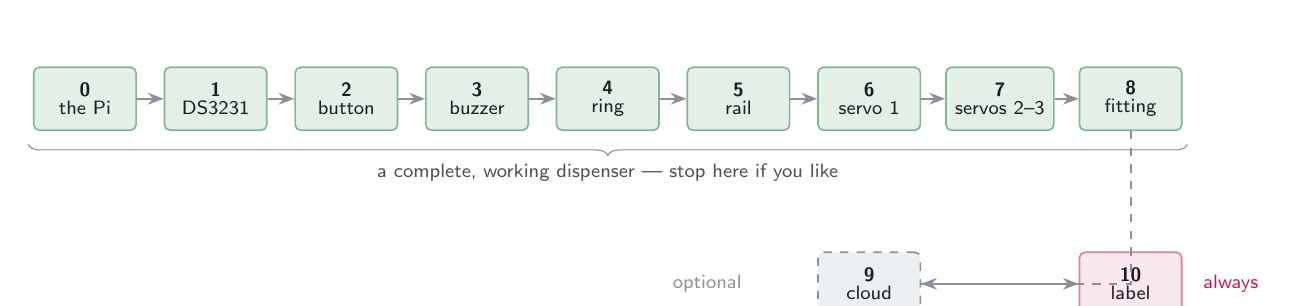
\begin{tikzpicture}[
   stg/.style={rounded corners=2pt, draw=ink40, fill=white, line width=0.6pt,
               minimum height=8mm, minimum width=13mm, font=\sffamily\scriptsize,
               align=center, text=ink},
   done/.style={stg, fill=okgreen!12, draw=okgreen!55},
   opt/.style={stg, fill=ink15!45, draw=ink40, dashed},
]
  \foreach \i/\lbl in {%
      0/{the Pi}, 1/{DS3231}, 2/{button}, 3/{buzzer}, 4/{ring},
      5/{rail}, 6/{servo 1}, 7/{servos 2--3}, 8/{fitting}}{
    \node[done] (s\i) at ({\i*1.66},0) {\textbf{\i}\\[-0.4ex]\lbl};
  }
  \foreach \i in {0,...,7}{
    \pgfmathtruncatemacro{\j}{\i+1}
    \draw[-{Stealth[length=2mm]}, ink40, line width=0.7pt] (s\i) -- (s\j);}

  \draw[decorate, decoration={brace, amplitude=4pt, mirror}, ink40]
       (-0.72,-0.58) -- (1.66*8+0.72,-0.58)
       node[midway, below=3.5pt, font=\sffamily\scriptsize, text=ink70]
       {a complete, working dispenser \textemdash{} stop here if you like};

  \node[opt] (s9)  at (1.66*6,-2.35) {\textbf{9}\\[-0.4ex]cloud};
  \node[stg, fill=scred!10, draw=scred!55] (s10) at (1.66*8,-2.35)
       {\textbf{10}\\[-0.4ex]label};
  \draw[-{Stealth[length=2mm]}, ink40, line width=0.7pt, dashed]
       (s8.south) |- (s9.east);
  \draw[-{Stealth[length=2mm]}, ink40, line width=0.7pt] (s9) -- (s10);
  \node[font=\sffamily\scriptsize, text=ink40, anchor=east] at (1.66*5.1,-2.35)
       {optional};
  \node[font=\sffamily\scriptsize, text=scred, anchor=west] at (1.66*8+0.8,-2.35)
       {always};
\end{tikzpicture}
\end{center}

\vspace{3mm}
\begin{center}
\small
\begin{tabular}{@{}c l l >{\raggedright\arraybackslash}p{62mm}@{}}
\toprule
& \hdr{Subsystem} & \hdr{Where it lands} & \hdr{What it is for} \\
\midrule
\swatch{i2cc}  & DS3231         & GPIO 2/3 (\iic) $+$ 3.3\,V & knows the time after a power cut \\
\swatch{ringc} & WS2812 ring    & GPIO 18, through 330\ohm   & green / blue / amber / violet \\
\swatch{buzzc} & piezo buzzer   & GPIO 23, through 100\ohm   & the sound that fetches a person from another room \\
\swatch{btnc}  & confirm button & GPIO 24 to GND             & internal pull-up, 20\,ms glitch filter \\
\swatch{servo} & 3 $\times$ SG90 & GPIO 17, 27, 22           & signal only \textemdash{} never power \\
\bottomrule
\end{tabular}
\end{center}

% ═══════════════════════════════════════════════════════════════════════════
\section{Bill of materials}
\markboth{Bill of materials}{Bill of materials}

\begin{center}
\small
\begin{longtable}{@{}c c >{\raggedright}p{42mm} >{\raggedright\arraybackslash}p{68mm}@{}}
\toprule
& \hdr{Qty} & \hdr{Part} & \hdr{Notes} \\
\midrule
\endhead
\iconpi     & 1 & Raspberry Pi 3B & Any Pi with the 40-pin header works; the pin map assumes a 3B \\
\iconsd     & 1 & microSD card, 8\,GB+ & Raspberry Pi OS \textbf{Bookworm or newer} \textemdash{} the firmware drives WiFi through NetworkManager \\
\iconpsu    & 1 & Pi power supply, 5\,V 2.5\,A & The official one. Servos do \textbf{not} come off this \\
\iconservo  & 3 & SG90 micro servo & One per fitted tray. The firmware handles eight \\
\iconpsu    & 1 & 5\,V supply, 2\,A or better & Separate, for the servos and the ring \\
\iconcap    & 1 & 1000\uF{} electrolytic, 10\,V+ & Across the servo rail, physically close to the servos \\
\iconring   & 1 & WS2812 / NeoPixel ring, 12\,px & 16 and 24 also work \textemdash{} set \code{RING\_PIXELS} \\
\iconres    & 1 & 330\ohm{} resistor & In the ring's data line, at the \textbf{ring} end \\
\iconbuzzer & 1 & Passive piezo buzzer & Passive, not an active beeper \textemdash{} see below \\
\iconres    & 1 & 100\ohm{} resistor & In series with the buzzer \\
\iconbutton & 1 & Momentary push button & Any normally-open button. No external resistor needed \\
\iconrtc    & 1 & DS3231 RTC module & With a coin cell fitted. Read the ZS-042 warning below \\
\iconwire   & \textemdash{} & Jumper wire, terminal blocks & Dupont leads are fine for the bench; solder or screw terminals for anything that gets carried \\
\iconcloud  & \textemdash{} & a relay, if you want cloud sync & \emph{Not a part.} One container, deployed once for all your devices \textemdash{} see \code{../cloud\_relay/}. Skip it and the dispenser is LAN-only \\
\bottomrule
\end{longtable}
\end{center}

\vspace{-2mm}
\begin{warnbox}
\warntitle{``Passive'' buzzer}
The firmware makes the tone itself \textemdash{} pigpio drives the pin as a
2.7\,kHz square wave (\code{indicators.Buzzer.beep}). An \emph{active} buzzer
contains its own oscillator and sounds at its own frequency the moment it sees a
voltage, so it will still make a noise here, just not the one that was chosen.
2.7\,kHz is where a small piezo is loudest and where age-related hearing loss
has bitten least, which is the whole reason the number is in \code{config.py}.

\vspace{1.5ex}
\begin{center}
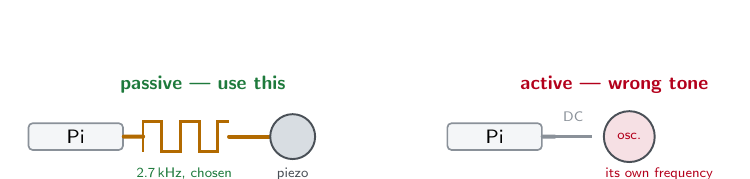
\begin{tikzpicture}[scale=0.95]
  % passive vs active
  \node[font=\sffamily\scriptsize\bfseries, text=okgreen] at (-2.6,1.05) {passive \textemdash{} use this};
  \node[font=\sffamily\scriptsize\bfseries, text=dangerred] at (2.9,1.05) {active \textemdash{} wrong tone};
  % passive: pi generates square wave
  \node[compbox, minimum width=12mm] (pa) at (-4.3,0.35) {Pi};
  \draw[wire, buzzc] (pa.east) -- (-3.4,0.35);
  \draw[buzzc, line width=1pt]
    (-3.4,0.15) -- (-3.4,0.55) -- (-3.15,0.55) -- (-3.15,0.15) -- (-2.9,0.15)
    -- (-2.9,0.55) -- (-2.65,0.55) -- (-2.65,0.15) -- (-2.4,0.15) -- (-2.4,0.55) -- (-2.25,0.55);
  \draw[wire, buzzc] (-2.25,0.35) -- (-1.7,0.35);
  \draw[ink70, line width=0.7pt, fill=ink15] (-1.4,0.35) circle (0.3);
  \node[font=\sffamily\tiny, text=ink70] at (-1.4,-0.15) {piezo};
  \node[font=\sffamily\tiny, text=okgreen] at (-2.85,-0.15) {2.7\,kHz, chosen};
  % active
  \node[compbox, minimum width=12mm] (ac) at (1.3,0.35) {Pi};
  \draw[wire, ink40] (ac.east) -- (2.1,0.35);
  \draw[ink40, line width=1pt] (2.1,0.35) -- (2.6,0.35);
  \node[font=\sffamily\tiny, text=ink40] at (2.35,0.62) {DC};
  \draw[ink70, line width=0.7pt, fill=dangerred!12] (3.1,0.35) circle (0.34);
  \node[font=\sffamily\tiny, text=dangerred] at (3.1,0.35) {osc.};
  \node[font=\sffamily\tiny, text=dangerred] at (3.5,-0.15) {its own frequency};
\end{tikzpicture}
\end{center}
\end{warnbox}

\begin{warnbox}
\warntitle{The DS3231 module and its coin cell}
The commonly sold ZS-042 board has a charging circuit intended for a
rechargeable LIR2032. Fitted with an ordinary non-rechargeable CR2032
\textemdash{} which is what most of them ship next to \textemdash{} it trickles
current into a cell that cannot take it. The usual fix is to remove the series
resistor in that charging path (marked \code{201} on most boards) or to use an
LIR2032. Either way, \textbf{fit the cell before the first
\code{hwclock -{}-systohc}}, because the whole point of the chip is what it
remembers with the power off.
\end{warnbox}

\clearpage

% ═══════════════════════════════════════════════════════════════════════════
\section{The header, and every pin this build touches}
\label{sec:header}

Keep this page open while you wire. Everything is BCM numbering, which is what
pigpio and RPi.GPIO both use; the small number inside each pad is the
\emph{physical} pin, which is what you actually count on the board.

\vspace{3mm}
\begin{center}
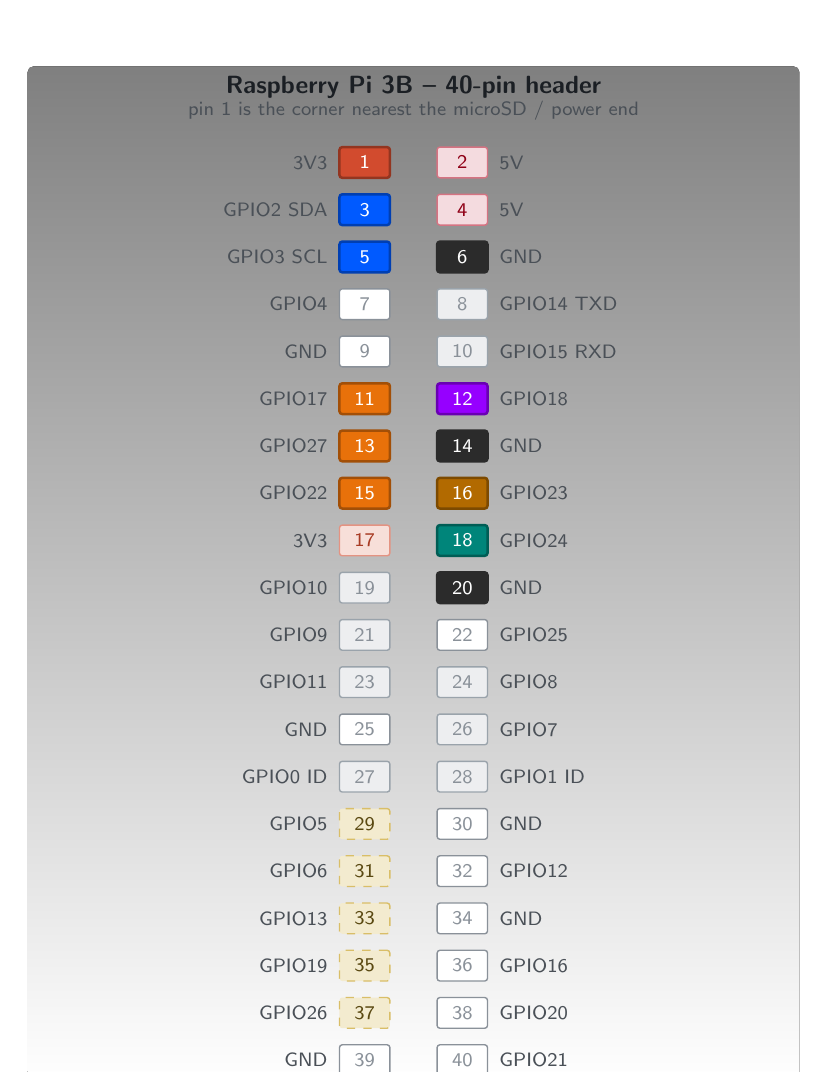
\begin{tikzpicture}[scale=1.0]
  \drawheader[0.60]
\end{tikzpicture}

\vspace{4mm}
\headerlegend
\end{center}

\vspace{4mm}
\begin{multicols}{2}
\noindent\textbf{\sffamily The pins that were avoided, and what each costs}

\vspace{1ex}
\footnotesize
\begin{tabular}{@{}>{\raggedright}p{20mm} >{\raggedright\arraybackslash}p{48mm}@{}}
\toprule
\hdr{Pin} & \hdr{Why it is not used} \\
\midrule
GPIO 0, 1 & HAT ID EEPROM. Driving them is how a HAT you plug in later fails to be detected \\
GPIO 2, 3 & Permanent 1.8\,k\textohm{} \iic{} pull-ups \textemdash{} a servo line idling high slams the horn at power-on. Now the DS3231 lives here \\
GPIO 14, 15 & The serial console: the one way back into a Pi whose network setup you just broke \\
GPIO 7--11 & SPI. Free today, gone the moment anyone adds an SPI display \\
\bottomrule
\end{tabular}

\columnbreak

\noindent\textbf{\sffamily Reserved for trays 4--8}

\vspace{1ex}
\footnotesize
GPIO 5, 6, 13, 19 and 26 are already checked for clashes and for the pins that
cost hardware, so a fourth hopper is a plug and a number, not a re-derivation:

\vspace{1ex}
\begin{shell}
SNAPCARE_TRAYS=8 python3 -m snapcare_dispenser
\end{shell}

\code{tests/test\_servo.py} asserts all of this, and that no peripheral shares a
pin with a servo.
\end{multicols}

\clearpage

% ═══════════════════════════════════════════════════════════════════════════
\section{Stage 0 \textemdash{} the Pi, before anything is wired to it}

Do this stage first because it is the only one that can be done comfortably with
the Pi on a desk and a keyboard attached. Once the servos are on it, every
mistake costs a power-down.

\begin{center}
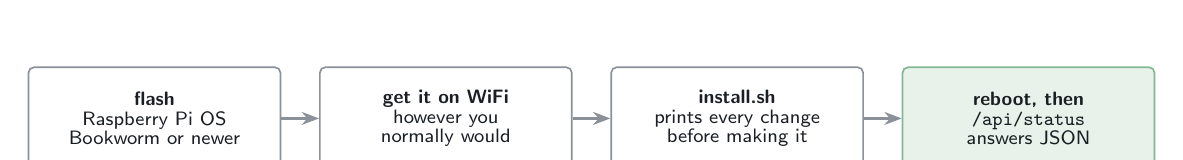
\begin{tikzpicture}[
  flowstep/.style={rounded corners=2pt, draw=ink40, fill=white, line width=0.6pt,
               minimum height=13mm, minimum width=32mm, align=center,
               font=\sffamily\scriptsize, text=ink},
]
  \node[flowstep] (a) at (0,0)    {\textbf{flash}\\[-0.3ex]Raspberry Pi OS\\[-0.3ex]Bookworm or newer};
  \node[flowstep] (b) at (3.7,0)  {\textbf{get it on WiFi}\\[-0.3ex]however you\\[-0.3ex]normally would};
  \node[flowstep] (c) at (7.4,0)  {\textbf{install.sh}\\[-0.3ex]prints every change\\[-0.3ex]before making it};
  \node[flowstep, fill=okgreen!10, draw=okgreen!55] (d) at (11.1,0)
       {\textbf{reboot, then}\\[-0.3ex]\code{/api/status}\\[-0.3ex]answers JSON};
  \foreach \x/\y in {a/b,b/c,c/d}{
    \draw[-{Stealth[length=2.2mm]}, ink40, line width=0.8pt] (\x) -- (\y);}
\end{tikzpicture}
\end{center}

\begin{shell}
git clone <this repo> && cd h1-SnapCare/pill_dispenser/rpi_firmware
sudo ./service/install.sh
sudo reboot            # the installer will tell you if the I2C overlay needs one
\end{shell}

The installer is safe to re-run. It installs pigpio and enables \code{pigpiod},
sets the hostname to \code{pilldispenser} and publishes it over avahi, writes the
captive-portal DNS rule, turns on \iic{} with the \code{i2c-rtc,ds3231} overlay,
disables \code{fake-hwclock}, installs \code{python3-cryptography} for cloud
sync, and installs the systemd unit.

\begin{provebox}
\provetitle
\begin{shell}
systemctl status snapcare-dispenser
curl -s http://localhost/api/status
\end{shell}
You should get JSON. It will say the clock is untrusted and that no servo
hardware is present \textemdash{} both correct, nothing is wired yet. The
\code{cloud} object will say \code{unpaired}, which is also correct: no relay
has been named.
\end{provebox}

% ═══════════════════════════════════════════════════════════════════════════
\section{Stage 1 \textemdash{} the DS3231}

\begin{dangerbox}
\dangertitle{Power off first \textemdash{} every time}
Not ``put it to sleep''. Unplug it. Every wiring stage in this guide starts that
way, and this reminder is not repeated after this page.
\end{dangerbox}

\begin{center}
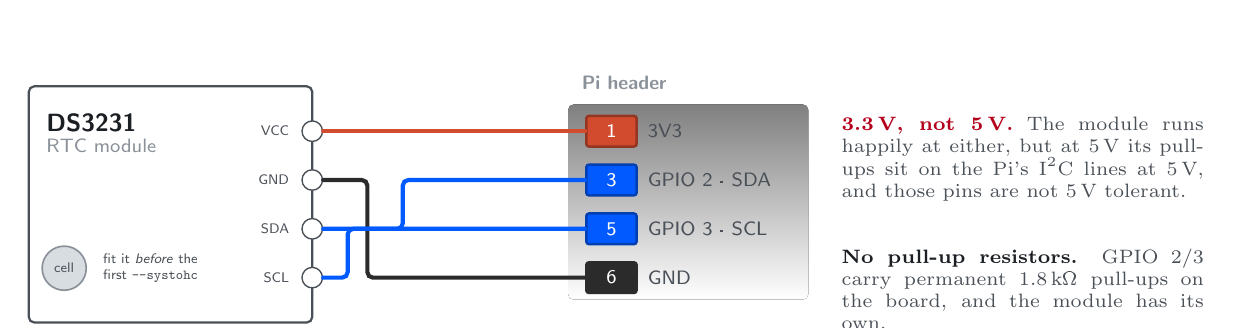
\begin{tikzpicture}
  % --- the module ---
  \node[modbox, minimum width=36mm, minimum height=30mm] (m) at (-3.7,-0.61) {};
  \node[modtitle, anchor=west] at (-5.4,0.42) {DS3231};
  \node[font=\sffamily\scriptsize, text=ink40, anchor=west] at (-5.4,0.14) {RTC module};
  \draw[ink40, line width=0.6pt, fill=ink15] (-5.05,-1.42) circle (0.28);
  \node[font=\sffamily\tiny, text=ink70] at (-5.05,-1.42) {cell};
  \node[font=\sffamily\tiny, text=ink70, align=left, anchor=west] at (-4.68,-1.42)
       {fit it \emph{before} the\\first \code{--systohc}};

  % terminals on the module's right edge
  \foreach \i/\nm in {0/VCC, 1/GND, 2/SDA, 3/SCL}{
    \pgfmathsetmacro{\ty}{0.32-\i*0.62}
    \node[term] (t\i) at (-1.9,\ty) {};
    \node[font=\sffamily\tiny, text=ink70, anchor=east] at (-2.07,\ty) {\nm};}

  % --- the header pads ---
  \hframe{1.9}{0.32}{-1.54}{Pi header}
  \hpin{1.9}{0.32}{1}{puse33}{3V3}
  \hpin{1.9}{-0.30}{3}{pusei2c}{GPIO 2 \textperiodcentered{} SDA}
  \hpin{1.9}{-0.92}{5}{pusei2c}{GPIO 3 \textperiodcentered{} SCL}
  \hpin{1.9}{-1.54}{6}{pusegnd}{GND}

  % --- wires ---
  \draw[wire, p33]  (t0) -- (H1.west);
  \draw[wire, gndc] (t1) -- (-1.2,-0.30) -- (-1.2,-1.54) -- (H6.west);
  \draw[wire, i2cc] (t2) -- (-0.75,-0.92) -- (-0.75,-0.30) -- (H3.west);
  \draw[wire, i2cc] (t3) -- (-1.45,-1.54) -- (-1.45,-0.92) -- (H5.west);

  % --- the 5 V trap ---
  \node[anchor=north west] at (4.7,0.62)
       {\begin{minipage}{46mm}\scriptsize\color{ink70}
        \textbf{\color{dangerred}3.3\,V, not 5\,V.} The module runs happily at
        either, but at 5\,V its pull-ups sit on the Pi's \iic{} lines at 5\,V,
        and those pins are not 5\,V tolerant.\end{minipage}};
  \node[anchor=north west] at (4.7,-1.05)
       {\begin{minipage}{46mm}\scriptsize\color{ink70}
        \textbf{\color{ink}No pull-up resistors.}
        GPIO 2/3 carry permanent 1.8\,k\textohm{} pull-ups on the board, and the
        module has its own.\end{minipage}};
\end{tikzpicture}
\end{center}

\vspace{-1mm}
\begin{center}\footnotesize\color{ink40}\sffamily
Physical pin numbers are in the pads. For where each one sits on the board, see
the header map on page~\pageref{sec:header}.
\end{center}

\begin{notebox}
That permanent pull-up is also exactly why GPIO 2 and 3 are kept out of the
servo map: a servo signal line that idles high before the software starts slams
the horn to one end at power-on, with a loaded tray on it.
\end{notebox}

\begin{provebox}
\provetitle
\begin{shell}
sudo i2cdetect -y 1        # expect 68 (and often 57, the EEPROM beside it)
ls -l /dev/rtc0            # the kernel overlay claimed it
sudo hwclock -r            # what the chip believes
sudo hwclock --systohc     # once the Pi's own time is right, write it in
\end{shell}
Then confirm the firmware agrees the clock can be \emph{believed}, which is a
different question from whether the chip is there:
\begin{shell}
curl -s http://localhost/api/status     # the "clock" object: trusted, source, rtc
\end{shell}
\end{provebox}

\begin{warnbox}
\warntitle{A dead cell does not make the chip vanish from the bus}
It makes it answer promptly with nonsense. The firmware reads the
oscillator-stop flag (bit 7 of register \code{0x0F}) and only a clear flag
counts. If it reads \code{untrusted} here with a good cell fitted, set the time
once through the API and it will clear the flag in the right order:
\begin{shell}
curl -X POST http://localhost/api/clock -d '{"iso":"2026-07-29T09:15:00"}'
\end{shell}
\end{warnbox}

% ═══════════════════════════════════════════════════════════════════════════
\section{Stage 2 \textemdash{} the confirm button}

Two wires, nothing else.

\begin{center}
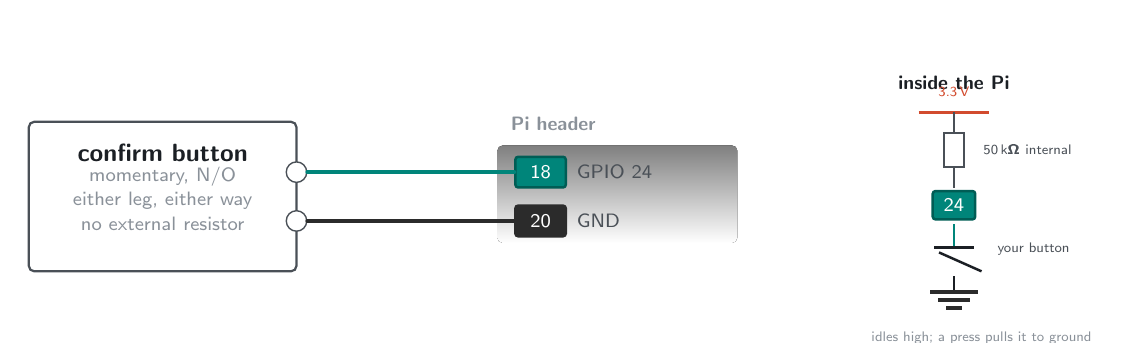
\begin{tikzpicture}
  % --- the button ---
  \node[modbox, minimum width=34mm, minimum height=19mm] (m) at (-4.2,-0.25) {};
  \node[modtitle] at (-4.2,0.3) {confirm button};
  \node[font=\sffamily\scriptsize, text=ink40] at (-4.2,0.0) {momentary, N/O};
  \node[font=\sffamily\scriptsize, text=ink40] at (-4.2,-0.3) {either leg, either way};
  \node[font=\sffamily\scriptsize, text=ink40] at (-4.2,-0.6) {no external resistor};

  \node[term] (t0) at (-2.5,0.06) {};
  \node[term] (t1) at (-2.5,-0.56) {};

  \hframe{0.6}{0.06}{-0.56}{Pi header}
  \hpin{0.6}{0.06}{18}{pusebtn}{GPIO 24}
  \hpin{0.6}{-0.56}{20}{pusegnd}{GND}

  \draw[wire, btnc]  (t0) -- (H18.west);
  \draw[wire, gndc]  (t1) -- (H20.west);

  % --- inset: the internal pull-up, and why no resistor is needed ---
  \begin{scope}[shift={(5.3,-0.3)}]
    \node[font=\sffamily\scriptsize\bfseries, text=ink] at (0.55,1.5) {inside the Pi};
    \draw[p33, line width=1pt] (0.1,1.12) -- (1.0,1.12);
    \node[font=\sffamily\tiny, text=p33, anchor=south] at (0.55,1.2) {3.3\,V};
    \draw[ink70, line width=0.7pt] (0.55,1.12) -- (0.55,0.86);
    \draw[ink70, line width=0.7pt, fill=white] (0.42,0.86) rectangle (0.68,0.42);
    \node[font=\sffamily\tiny, text=ink70, anchor=west] at (0.8,0.64) {50\,k\textohm{} internal};
    \draw[ink70, line width=0.7pt] (0.55,0.42) -- (0.55,0.16);
    \node[pusebtn, minimum width=5.4mm, minimum height=3.6mm] at (0.55,-0.06) {24};
    \draw[btnc, line width=1pt] (0.55,-0.3) -- (0.55,-0.6);
    % the switch
    \draw[ink, line width=0.9pt] (0.3,-0.6) -- (0.8,-0.6);
    \draw[ink, line width=0.9pt] (0.36,-0.66) -- (0.9,-0.9);
    \draw[ink, line width=0.9pt] (0.55,-0.96) -- (0.55,-1.16);
    \node[font=\sffamily\tiny, text=ink70, anchor=west] at (0.98,-0.62) {your button};
    \draw[gndc, line width=1.4pt] (0.25,-1.16) -- (0.85,-1.16);
    \draw[gndc, line width=1.4pt] (0.35,-1.26) -- (0.75,-1.26);
    \draw[gndc, line width=1.4pt] (0.45,-1.36) -- (0.65,-1.36);
    \node[font=\sffamily\tiny, text=ink40, align=center, anchor=north] at (0.9,-1.55)
         {idles high; a press pulls it to ground};
  \end{scope}
\end{tikzpicture}
\end{center}

\vspace{1mm}
\noindent\textbf{\sffamily Why there is no debounce capacitor.} A real switch
does not close once; it chatters for a few milliseconds. Pigpio's glitch filter
discards any edge that does not then hold for 20\,ms
(\code{BUTTON\_DEBOUNCE\_US}), \emph{before} a callback is ever queued.
Undebounced, one press records several doses.

\vspace{2mm}
\begin{center}
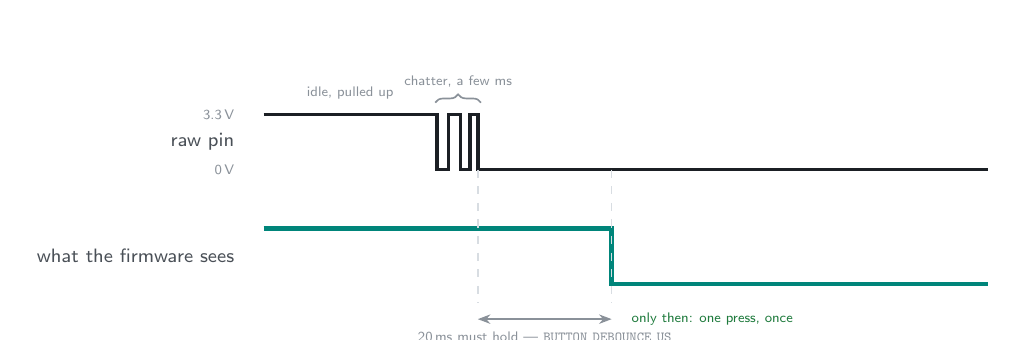
\begin{tikzpicture}[scale=1]
  \node[font=\sffamily\scriptsize, text=ink70, anchor=east] at (-0.25,0.5) {raw pin};
  \node[font=\sffamily\scriptsize, text=ink70, anchor=east] at (-0.25,-0.95)
       {what the firmware sees};
  \node[font=\sffamily\tiny, text=ink40, anchor=east] at (-0.25,0.85) {3.3\,V};
  \node[font=\sffamily\tiny, text=ink40, anchor=east] at (-0.25,0.15) {0\,V};

  % raw: idles high, chatters, settles low
  \draw[ink, line width=1.3pt]
    (0,0.85) -- (2.2,0.85) -- (2.2,0.15) -- (2.35,0.15) -- (2.35,0.85) -- (2.5,0.85)
    -- (2.5,0.15) -- (2.62,0.15) -- (2.62,0.85) -- (2.72,0.85) -- (2.72,0.15)
    -- (9.2,0.15);
  \draw[decorate, decoration={brace, amplitude=3pt}, ink40, line width=0.6pt]
    (2.18,1.0) -- (2.76,1.0)
    node[midway, above=2pt, font=\sffamily\tiny, text=ink40] {chatter, a few ms};
  \node[font=\sffamily\tiny, text=ink40, anchor=south] at (1.1,0.92) {idle, pulled up};

  % filtered
  \draw[btnc, line width=1.6pt]
    (0,-0.6) -- (4.42,-0.6) -- (4.42,-1.3) -- (9.2,-1.3);
  \draw[ink15, line width=0.6pt, dashed] (2.72,0.15) -- (2.72,-1.55);
  \draw[ink15, line width=0.6pt, dashed] (4.42,0.15) -- (4.42,-1.55);
  \draw[{Stealth[length=1.6mm]}-{Stealth[length=1.6mm]}, ink40, line width=0.5pt]
       (2.72,-1.75) -- (4.42,-1.75)
       node[midway, below=1pt, font=\sffamily\tiny, text=ink40]
       {20\,ms must hold \textemdash{} \code{BUTTON\_DEBOUNCE\_US}};
  \node[font=\sffamily\tiny, text=okgreen, anchor=west] at (4.55,-1.75)
       {only then: one press, once};
\end{tikzpicture}
\end{center}

\begin{provebox}
\provetitle
You need a dose waiting to confirm, so this is easiest tested at the end of
Stage 3 \textemdash{} but you can check the firmware claimed the pin now:
\begin{shell}
journalctl -u snapcare-dispenser | grep -i button
\end{shell}
It should report the \code{pigpio} backend. \code{poll} means pigpiod is not
running, and \code{none} means neither is available.
\end{provebox}

% ═══════════════════════════════════════════════════════════════════════════
\section{Stage 3 \textemdash{} the buzzer}

\begin{center}
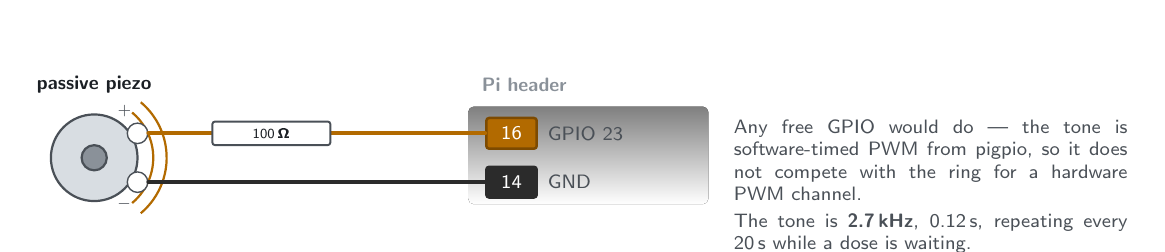
\begin{tikzpicture}
  \draw[ink70, line width=0.8pt, fill=ink15] (-3.4,-0.25) circle (0.55);
  \draw[ink70, line width=0.8pt, fill=ink40] (-3.4,-0.25) circle (0.16);
  \node[font=\sffamily\scriptsize\bfseries, text=ink, anchor=south] at (-3.4,0.45)
       {passive piezo};
  \foreach \r in {0.75,0.92}{
    \draw[buzzc, line width=0.8pt] (-3.4,-0.25) ++(-50:\r) arc (-50:50:\r);}

  \node[term] (tp) at (-2.85,0.06) {};
  \node[font=\sffamily\tiny, text=ink70, anchor=south east] at (-2.8,0.14) {$+$};
  \node[term] (tm) at (-2.85,-0.56) {};
  \node[font=\sffamily\tiny, text=ink70, anchor=north east] at (-2.8,-0.64) {$-$};

  \hframe{1.9}{0.06}{-0.56}{Pi header}
  \hpin{1.9}{0.06}{16}{pusebuzz}{GPIO 23}
  \hpin{1.9}{-0.56}{14}{pusegnd}{GND}

  \coordinate (ra) at (-1.9,0.06);
  \coordinate (rb) at (-0.4,0.06);
  \draw[wire, buzzc] (tp) -- (ra);
  \draw[wire, buzzc] (rb) -- (H16.west);
  \draw[ink70, line width=0.7pt, fill=white, rounded corners=1pt]
       (-1.9,-0.09) rectangle (-0.4,0.21);
  \node[font=\sffamily\tiny, text=ink] at (-1.15,0.06) {100\,\textohm};
  \draw[wire, gndc] (tm) -- (H14.west);

  \node[font=\sffamily\scriptsize, text=ink70, align=left, anchor=north west]
       at (4.6,0.35)
       {\begin{minipage}{50mm}\scriptsize Any free GPIO would do \textemdash{}
        the tone is software-timed PWM from pigpio, so it does not compete with
        the ring for a hardware PWM channel.\\[0.6ex]
        The tone is \textbf{2.7\,kHz}, 0.12\,s, repeating every 20\,s while a
        dose is waiting.\end{minipage}};
\end{tikzpicture}
\end{center}

\begin{provebox}
\provetitle
\begin{shell}
curl -X POST http://localhost/api/drop -d '{"tray":1}'
\end{shell}
With nothing else wired this drops a tray that does not exist yet, which is
fine \textemdash{} what you are listening for is the chirp that starts when the
dose goes into the confirm state, repeating every 20\,s. \textbf{Press the
button to stop it}, which tests Stage 2 at the same time. If it will not stop,
the button is the problem; if nothing sounds, the buzzer is.
\end{provebox}

% ═══════════════════════════════════════════════════════════════════════════
\section{Stage 4 \textemdash{} the LED ring}

This is the first stage that touches the servo supply. The ring's 5\,V does
\emph{not} come from the Pi.

\begin{center}
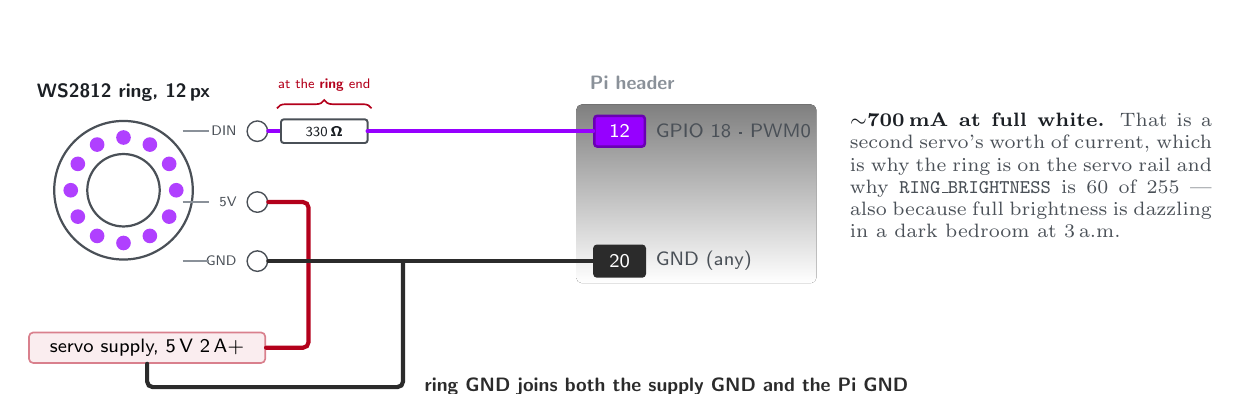
\begin{tikzpicture}
  % --- the ring ---
  \begin{scope}[shift={(-4.7,-0.6)}]
    \draw[ink70, line width=0.8pt] (0,0) circle (0.88);
    \draw[ink70, line width=0.8pt] (0,0) circle (0.46);
    \foreach \a in {0,30,...,330}{\fill[ringc!75] (\a:0.67) circle (0.093);}
    \node[font=\sffamily\scriptsize\bfseries, text=ink, anchor=south] at (0,1.0)
         {WS2812 ring, 12\,px};
  \end{scope}
  % leads off the ring's rim
  \node[term] (din) at (-3.0,0.15) {};
  \node[font=\sffamily\tiny, text=ink70, anchor=east] at (-3.14,0.15) {DIN};
  \node[term] (r5) at (-3.0,-0.75) {};
  \node[font=\sffamily\tiny, text=ink70, anchor=east] at (-3.14,-0.75) {5V};
  \node[term] (rg) at (-3.0,-1.5) {};
  \node[font=\sffamily\tiny, text=ink70, anchor=east] at (-3.14,-1.5) {GND};
  \draw[ink40, line width=0.6pt] (-3.95,0.15) -- (-3.62,0.15);
  \draw[ink40, line width=0.6pt] (-3.95,-0.75) -- (-3.62,-0.75);
  \draw[ink40, line width=0.6pt] (-3.95,-1.5) -- (-3.62,-1.5);

  % --- header pads first, so wires can anchor to them ---
  \hframe{1.6}{0.15}{-1.5}{Pi header}
  \hpin{1.6}{0.15}{12}{pusering}{GPIO 18 \textperiodcentered{} PWM0}
  \hpin{1.6}{-1.5}{20}{pusegnd}{GND (any)}

  % --- 330 ohm, hard against the ring ---
  \draw[wire, ringc] (din) -- (-2.7,0.15);
  \draw[ink70, line width=0.7pt, fill=white, rounded corners=1pt]
       (-2.7,0.0) rectangle (-1.6,0.3);
  \node[font=\sffamily\tiny, text=ink] at (-2.15,0.15) {330\,\textohm};
  \draw[wire, ringc] (-1.6,0.15) -- (H12.west);

  \draw[decorate, decoration={brace, amplitude=3pt}, dangerred, line width=0.6pt]
       (-2.75,0.44) -- (-1.55,0.44)
       node[midway, above=2.5pt, font=\sffamily\tiny, text=dangerred]
       {at the \textbf{ring} end};

  \node[compbox, minimum width=30mm, fill=p5!7, draw=p5!50] (rail) at (-4.4,-2.6)
       {servo supply, 5\,V 2\,A$+$};
  \draw[wire, p5]   (r5) -- (-2.35,-0.75) -- (-2.35,-2.6) -- (rail.east);
  \draw[wire, gndc] (rg) -- (-1.15,-1.5) -- (H20.west);
  \draw[wire, gndc] (-1.15,-1.5) -- (-1.15,-3.1) -- (-4.4,-3.1) -- (rail.south);
  \node[font=\sffamily\scriptsize\bfseries, text=gndc, anchor=west] at (-1.0,-3.1)
       {ring GND joins \emph{both} the supply GND and the Pi GND};

  \node[anchor=north west] at (4.4,0.5)
       {\begin{minipage}{46mm}\scriptsize\color{ink70}
        \textbf{\color{ink}$\sim$700\,mA at full white.} That is a second
        servo's worth of current, which is why the ring is on the servo rail and
        why \code{RING\_BRIGHTNESS} is 60 of 255 \textemdash{} also because full
        brightness is dazzling in a dark bedroom at 3\,a.m.\end{minipage}};
\end{tikzpicture}
\end{center}

\begin{dangerbox}
\dangertitle{GPIO 18 is not a free choice}
\code{rpi\_ws281x} generates the WS2812's 800\,kHz waveform with the PWM or PCM
peripheral and the DMA controller, and \textbf{GPIO 18, 12, 21 and 10 are the
only pins wired to them.} Anything else is a ring that never lights and an error
message about DMA. GPIO 18 is PWM0 and is not in the servo map. A test asserts
this (\code{tests/test\_servo.py:181}).
\end{dangerbox}

\noindent\textbf{\sffamily The 330\,\textohm{} is not folklore.} It damps the
reflection on the first data edge, which is what makes the first pixel latch a
wrong colour on a long lead. It has to be at the ring end to do that.

\begin{provebox}
\provetitle
\begin{shell}
sudo systemctl restart snapcare-dispenser
curl -s http://localhost/api/status     # "indicators" should now list the ring
curl -X POST http://localhost/api/schedule \
     -H 'Content-Type: application/json' \
     -d '{"payload":"SC1*W*1:0800-127-030"}'   # violet: schedule accepted
\end{shell}
If the ring stays dark, check \code{journalctl} \textemdash{} a ring that throws
is dropped and logged rather than retried forever, and the status page reports
what is actually fitted rather than pretending.
\end{provebox}

\vspace{2mm}
\noindent\textbf{\sffamily The colour vocabulary you have just fitted.} Never
text, because the person the machine is for cannot be assumed to read.

\vspace{2mm}
\begin{center}

\begin{tikzpicture}
  \foreach \i/\col/\ttl/\sub in {%
      0/ledgreen/{dose ready}/{$+$ chirp},
      1/ledblue/{dose taken}/{button pressed},
      2/ledamber/{dose missed}/{grace ran out},
      3/ledviolet/{new schedule}/{accepted},
      4/ledcyan/{needs a network}/{join its hotspot}}{
    \pgfmathsetmacro{\x}{\i*2.85}
    \begin{scope}[shift={(\x,0)}]
      \draw[ink15, line width=0.6pt] (0,0) circle (0.42);
      \foreach \a in {0,30,...,330}{\fill[\col] (\a:0.32) circle (0.055);}
      \node[font=\sffamily\scriptsize\bfseries, text=ink, anchor=west] at (0.58,0.12) {\ttl};
      \node[font=\sffamily\scriptsize, text=ink40, anchor=west] at (0.58,-0.14) {\sub};
    \end{scope}}
\end{tikzpicture}
\end{center}

% ═══════════════════════════════════════════════════════════════════════════
\section{Stage 5 \textemdash{} the servo power rail, before any servo}

Wire and measure the rail with \textbf{no servos attached and no signal wires to
the Pi}. This is the stage that protects the SD card.

\begin{center}
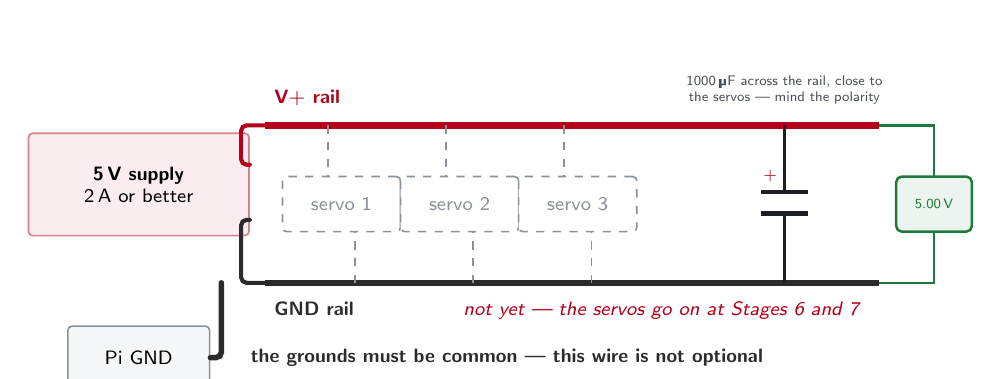
\begin{tikzpicture}
  % --- supply ---
  \node[compbox, minimum width=28mm, minimum height=13mm, fill=p5!7, draw=p5!50]
       (psu) at (-4.9,-0.75) {\textbf{5\,V supply}\\ 2\,A or better};

  % --- the two rails ---
  \draw[p5, line width=2.4pt] (-3.3,0) -- (4.5,0);
  \node[font=\sffamily\scriptsize\bfseries, text=p5, anchor=south west] at (-3.3,0.12) {V$+$ rail};
  \draw[gndc, line width=2.4pt] (-3.3,-2.0) -- (4.5,-2.0);
  \node[font=\sffamily\scriptsize\bfseries, text=gndc, anchor=north west] at (-3.3,-2.12) {GND rail};

  \draw[wire, p5]   (psu.east|-0,-0.5) -- (-3.6,-0.5) -- (-3.6,0) -- (-3.3,0);
  \draw[wire, gndc] (psu.east|-0,-1.2) -- (-3.6,-1.2) -- (-3.6,-2.0) -- (-3.3,-2.0);

  % --- bulk capacitor, close to the servos ---
  \draw[ink, line width=1.1pt] (3.3,0) -- (3.3,-0.85);
  \draw[ink, line width=1.6pt] (3.0,-0.85) -- (3.6,-0.85);
  \draw[ink, line width=1.6pt] (3.0,-1.12) -- (3.6,-1.12);
  \draw[ink, line width=1.1pt] (3.3,-1.12) -- (3.3,-2.0);
  \node[font=\sffamily\tiny, text=p5] at (3.12,-0.64) {$+$};
  \node[font=\sffamily\tiny, text=ink70, anchor=south, align=center] at (3.3,0.14)
       {1000\uF{} across the rail, close to\\the servos \textemdash{} mind the polarity};

  % --- three servo taps, deliberately empty ---
  \foreach \i/\x in {1/-2.5, 2/-1.0, 3/0.5}{
    \draw[ink40, dashed, line width=0.7pt] (\x,0) -- (\x,-0.72);
    \draw[ink40, dashed, line width=0.7pt] (\x+0.35,-2.0) -- (\x+0.35,-1.28);
    \node[compbox, minimum width=15mm, minimum height=7mm, draw=ink40, dashed,
          fill=white, text=ink40] at (\x+0.175,-1.0) {servo \i};}
  \node[font=\sffamily\scriptsize\itshape, text=dangerred, anchor=north west]
       at (-0.9,-2.12) {not yet \textemdash{} the servos go on at Stages 6 and 7};

  % --- the Pi's ground, which is the whole point ---
  \node[compbox, minimum width=18mm, minimum height=8mm] (pig) at (-4.9,-2.95)
       {Pi GND};
  \draw[wire, gndc, line width=2pt] (pig.east) -- (-3.85,-2.95) -- (-3.85,-2.0);
  \node[font=\sffamily\scriptsize\bfseries, text=gndc, anchor=west] at (-3.6,-2.95)
       {the grounds must be common \textemdash{} this wire is not optional};

  % --- meter ---
  \draw[okgreen, line width=0.9pt] (4.5,0) -- (5.2,0) -- (5.2,-0.65);
  \draw[okgreen, line width=0.9pt] (4.5,-2.0) -- (5.2,-2.0) -- (5.2,-1.35);
  \draw[okgreen, line width=0.9pt, fill=okgreen!8, rounded corners=2pt]
       (4.72,-1.35) rectangle (5.68,-0.65);
  \node[font=\sffamily\tiny, text=okgreen] at (5.2,-1.0) {5.00\,V};
\end{tikzpicture}
\end{center}

\begin{dangerbox}
\dangertitle{Do not run the servos from the Pi's 5\,V pin}
One SG90 stalls at around 700\,mA. The failure is not a blown regulator; it is a
brown-out, and \textbf{a Pi that browns out mid-write corrupts an SD card}
\textemdash{} where the file being written is the one that records whether a
dose has already been given.
\end{dangerbox}

\noindent The common ground is what makes the signal mean anything. Without it
the servos twitch or ignore commands entirely, which reads as a firmware fault
and is not one. The bulk capacitor absorbs the current step when a servo starts,
which is what otherwise dips the rail.

\begin{provebox}
\provetitle
Meter across the rail. \textbf{5\,V $\pm$0.25\,V, steady.} Nothing else is
connected yet, so anything else is the supply or the wiring, not the firmware.
\end{provebox}

% ═══════════════════════════════════════════════════════════════════════════
\section{Stage 6 \textemdash{} one servo}

Do one, entirely, before the other two.

\begin{center}
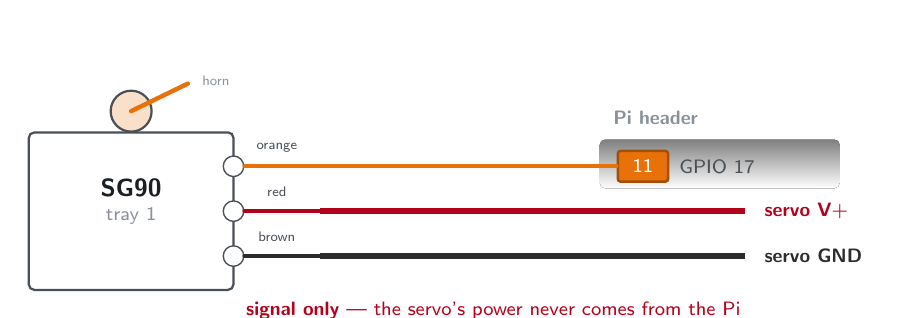
\begin{tikzpicture}
  % --- the servo ---
  \node[modbox, minimum width=26mm, minimum height=20mm] (s) at (-4.9,-0.72) {};
  \node[modtitle] at (-4.9,-0.42) {SG90};
  \node[font=\sffamily\scriptsize, text=ink40] at (-4.9,-0.78) {tray 1};
  \draw[ink70, line width=0.8pt, fill=servo!22] (-4.9,0.55) circle (0.26);
  \draw[servo, line width=1.6pt, line cap=round] (-4.9,0.55) -- (-4.18,0.9);
  \node[font=\sffamily\tiny, text=ink40, anchor=west] at (-4.12,0.94) {horn};

  % three leads, in the colours the part actually uses
  \node[term] (sg) at (-3.6,-0.15) {};
  \node[term] (sv) at (-3.6,-0.72) {};
  \node[term] (sn) at (-3.6,-1.29) {};
  \node[font=\sffamily\tiny, text=ink70, anchor=south] at (-3.05,-0.09) {orange};
  \node[font=\sffamily\tiny, text=ink70, anchor=south] at (-3.05,-0.66) {red};
  \node[font=\sffamily\tiny, text=ink70, anchor=south] at (-3.05,-1.23) {brown};

  % --- header pad ---
  \hframe{1.6}{-0.15}{-0.15}{Pi header}
  \hpin{1.6}{-0.15}{11}{puseservo}{GPIO 17}
  \draw[wire, servo] (sg) -- (H11.west);
  \node[font=\sffamily\scriptsize, text=dangerred, anchor=north] at (-0.3,-1.75)
       {\textbf{signal only} \textemdash{} the servo's power never comes from the Pi};

  % --- the rail from stage 5 ---
  \draw[p5, line width=2.2pt] (-2.5,-0.72) -- (2.9,-0.72);
  \draw[gndc, line width=2.2pt] (-2.5,-1.29) -- (2.9,-1.29);
  \node[font=\sffamily\scriptsize\bfseries, text=p5, anchor=west] at (3.02,-0.72) {servo V$+$};
  \node[font=\sffamily\scriptsize\bfseries, text=gndc, anchor=west] at (3.02,-1.29) {servo GND};
  \draw[wire, p5] (sv) -- (-2.5,-0.72);
  \draw[wire, gndc] (sn) -- (-2.5,-1.29);
\end{tikzpicture}
\end{center}

\begin{provebox}
\provetitle
\begin{shell}
sudo systemctl restart snapcare-dispenser
curl -X POST http://localhost/api/drop -d '{"tray":1}'
\end{shell}
One sweep: rest at 0\dgr, out to 180\dgr, back to 0\dgr, about a second in
total. Then the signal to that pin is \textbf{cut} rather than held \textemdash{}
so the servo should go silent and cool between doses.
\end{provebox}

\vspace{1mm}
\begin{center}
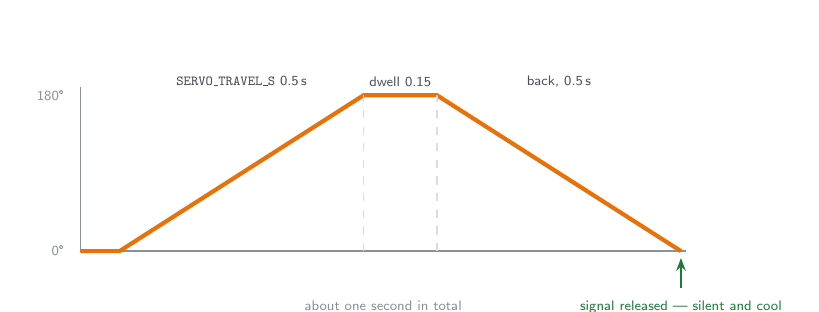
\begin{tikzpicture}[xscale=6.2, yscale=0.011]
  % axes
  \draw[ink40, line width=0.5pt] (0,0) -- (1.24,0);
  \draw[ink40, line width=0.5pt] (0,0) -- (0,190);
  \node[font=\sffamily\tiny, text=ink40, anchor=east] at (-0.012,0) {0\dgr};
  \node[font=\sffamily\tiny, text=ink40, anchor=east] at (-0.012,180) {180\dgr};
  % the sweep
  \draw[servo, line width=1.5pt]
    (0,0) -- (0.08,0) -- (0.58,180) -- (0.73,180) -- (1.23,0);
  \draw[ink15, line width=0.5pt, dashed] (0.58,0) -- (0.58,180);
  \draw[ink15, line width=0.5pt, dashed] (0.73,0) -- (0.73,180);
  % annotations
  \node[font=\sffamily\tiny, text=ink70] at (0.33,196) {\code{SERVO\_TRAVEL\_S} 0.5\,s};
  \node[font=\sffamily\tiny, text=ink70] at (0.655,196) {dwell 0.15};
  \node[font=\sffamily\tiny, text=ink70] at (0.98,196) {back, 0.5\,s};
  \draw[-{Stealth[length=1.6mm]}, okgreen, line width=0.8pt] (1.23,-42) -- (1.23,-8);
  \node[font=\sffamily\tiny, text=okgreen, anchor=north] at (1.23,-46)
       {signal released \textemdash{} silent and cool};
  \node[font=\sffamily\tiny, text=ink40, anchor=north] at (0.62,-46) {about one second in total};
\end{tikzpicture}
\end{center}

\vspace{2mm}
\noindent\textbf{\sffamily Check which driver you got.} \code{servoBackend} in
the status, with \code{servoSteady} saying whether its timing can be trusted:

\begin{shell}
curl -s http://localhost/api/status | grep -i servo
\end{shell}

\begin{center}
\small
\begin{tabular}{@{}l l >{\raggedright\arraybackslash}p{78mm}@{}}
\toprule
\hdr{Backend} & \hdr{Verdict} & \hdr{What it means} \\
\midrule
\code{pigpio} & \textcolor{okgreen}{\textbf{what you want}} & Pulses timed by the DMA controller, immune to CPU load \\
\code{rpigpio} & \textcolor{warnamber}{\textbf{jittery fallback}} & Pulses timed from a Python thread; every kernel preemption is a visible twitch and an audible buzz. Reports \code{servoSteady: false}. Fix with \code{sudo systemctl enable -{}-now pigpiod} \\
\code{mock} & \textcolor{dangerred}{\textbf{nothing moves}} & No servo library present at all \\
\bottomrule
\end{tabular}
\end{center}

% ═══════════════════════════════════════════════════════════════════════════
\section{Stage 7 \textemdash{} the other two servos}

\begin{center}
\begin{minipage}{0.36\textwidth}
\small
\begin{tabular}{@{}c c c@{}}
\toprule
\hdr{Tray} & \hdr{GPIO} & \hdr{Header pin} \\
\midrule
1 & 17 & 11 \\
2 & 27 & 13 \\
3 & 22 & 15 \\
\bottomrule
\end{tabular}
\end{minipage}\hfill
\begin{minipage}{0.58\textwidth}
\small
\code{INSTALLED\_TRAYS = 3} in \code{config.py} is the only thing that says
three. The map lists all eight, so scaling up is one number and some servos.
Trays 4--8 are reserved at GPIO 5, 6, 13, 19 and 26 \textemdash{} already
checked for clashes, so a fourth hopper is a plug and a number.
\end{minipage}
\end{center}

\vspace{2mm}
\begin{provebox}
\provetitle
Prove each one \emph{individually}, and watch which hopper actually moves:
\begin{shell}
for t in 1 2 3; do curl -X POST http://localhost/api/drop -d "{\"tray\":$t}"; sleep 2; done
\end{shell}
\end{provebox}

\begin{dangerbox}
\dangertitle{This is the one worth doing carefully}
Two trays on one pin gives the right number of pills from the wrong
compartment, and \textbf{nobody notices that until the wrong medication has been
taken for a week.} The firmware refuses a duplicate pin at startup, but it
cannot check that the wire you plugged into GPIO 27 goes to the hopper you are
calling tray 2.

\vspace{2ex}
\begin{center}
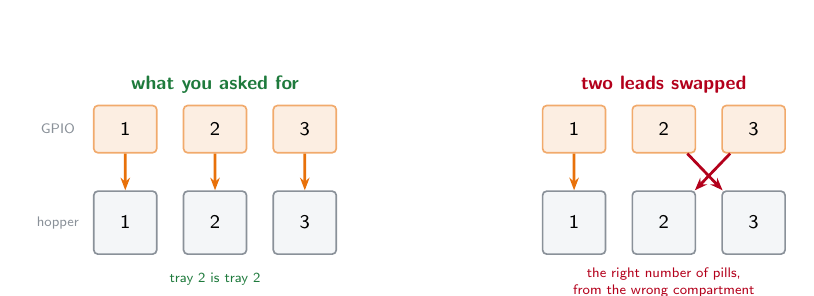
\begin{tikzpicture}[scale=0.95]
  % --- correct ---
  \node[font=\sffamily\scriptsize\bfseries, text=okgreen] at (-3.4,1.5) {what you asked for};
  \foreach \i/\x in {1/-4.6, 2/-3.4, 3/-2.2}{
    \node[pusesservoish/.try, compbox, minimum width=8mm, minimum height=6mm,
          fill=servo!12, draw=servo!60] (a\i) at (\x,0.9) {\i};
    \node[compbox, minimum width=8mm, minimum height=8mm] (b\i) at (\x,-0.35) {\i};}
  \foreach \i in {1,2,3}{\draw[servo, line width=1pt, -{Stealth[length=1.6mm]}] (a\i) -- (b\i);}
  \node[font=\sffamily\tiny, text=ink40] at (-5.5,0.9) {GPIO};
  \node[font=\sffamily\tiny, text=ink40] at (-5.5,-0.35) {hopper};
  \node[font=\sffamily\tiny, text=okgreen] at (-3.4,-1.1) {tray 2 is tray 2};

  % --- swapped ---
  \node[font=\sffamily\scriptsize\bfseries, text=dangerred] at (2.6,1.5) {two leads swapped};
  \foreach \i/\x in {1/1.4, 2/2.6, 3/3.8}{
    \node[compbox, minimum width=8mm, minimum height=6mm,
          fill=servo!12, draw=servo!60] (c\i) at (\x,0.9) {\i};
    \node[compbox, minimum width=8mm, minimum height=8mm] (d\i) at (\x,-0.35) {\i};}
  \draw[servo, line width=1pt, -{Stealth[length=1.6mm]}] (c1) -- (d1);
  \draw[dangerred, line width=1pt, -{Stealth[length=1.6mm]}] (c2) -- (d3);
  \draw[dangerred, line width=1pt, -{Stealth[length=1.6mm]}] (c3) -- (d2);
  \node[font=\sffamily\tiny, text=dangerred, align=center] at (2.6,-1.15)
       {the right number of pills,\\from the wrong compartment};
\end{tikzpicture}
\end{center}
\end{dangerbox}

\noindent\textbf{\sffamily Only one servo is ever driven at a time}, enforced by
a lock \textemdash{} three doses owed at the same minute still move one horn at a
time. Eight SG90s starting together is a current step that reboots the Pi with a
compartment open.

% ═══════════════════════════════════════════════════════════════════════════
\section{Stage 8 \textemdash{} mechanical fitting and trim}

Fit the hoppers with the servos at their \textbf{resting 0\dgr}, not wherever the
horn happened to stop. Park each one there first, then mount the horn:

\begin{shell}
sudo python3 -m snapcare_dispenser --drop 1     # sweeps, and ends at rest
\end{shell}

\begin{center}
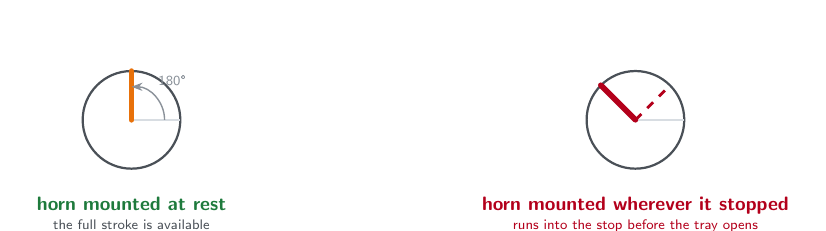
\begin{tikzpicture}
  % --- right ---
  \begin{scope}[shift={(-3.2,0)}]
    \draw[ink70, line width=0.8pt, fill=white] (0,0) circle (0.62);
    \draw[ink15, line width=0.5pt] (0,0) -- (0.62,0);
    \draw[servo, line width=2pt, line cap=round] (0,0) -- (0,0.62);
    \draw[ink40, line width=0.5pt, -{Stealth[length=1.4mm]}]
         (0.42,0) arc (0:90:0.42);
    \node[font=\sffamily\tiny, text=ink40] at (0.52,0.5) {180\dgr};
    \node[font=\sffamily\scriptsize\bfseries, text=okgreen, anchor=north] at (0,-0.85)
         {horn mounted at rest};
    \node[font=\sffamily\tiny, text=ink70, anchor=north, align=center] at (0,-1.15)
         {the full stroke is available};
  \end{scope}
  % --- wrong ---
  \begin{scope}[shift={(3.2,0)}]
    \draw[ink70, line width=0.8pt, fill=white] (0,0) circle (0.62);
    \draw[ink15, line width=0.5pt] (0,0) -- (0.62,0);
    \draw[dangerred, line width=2pt, line cap=round] (0,0) -- (-0.44,0.44);
    \draw[dangerred, line width=1pt, dashed] (0,0) -- (0.44,0.44);
    \node[font=\sffamily\scriptsize\bfseries, text=dangerred, anchor=north] at (0,-0.85)
         {horn mounted wherever it stopped};
    \node[font=\sffamily\tiny, text=dangerred, anchor=north, align=center] at (0,-1.15)
         {runs into the stop before the tray opens};
  \end{scope}
\end{tikzpicture}
\end{center}

\vspace{1mm}
If a tray does not quite reach its stop, or buzzes at the end of the stroke
because it is being driven past it, trim \emph{that tray alone}:

\begin{pycode}
SERVO_TRIM = {3: (520, 2450)}    # config.py -- overrides only tray 3
\end{pycode}

\begin{warnbox}
\warntitle{Buzzing at the end of a stroke is the one to act on}
It is the servo fighting a mechanical stop it has already reached, and it is
what burns one out over a few weeks.
\end{warnbox}

\noindent The other two knobs, if a full hopper is slower than an empty one:

\begin{pycode}
SERVO_TRAVEL_S = 0.5     # one traverse; open-loop, nothing reports arrival
SERVO_DWELL_S  = 0.15    # pause at the far end before returning
\end{pycode}

\noindent \code{SERVO\_TRAVEL\_S} must cover the \emph{slowest} case \textemdash{}
a cold servo under the weight of a full tray \textemdash{} because nothing on an
SG90 reports position and the firmware is simply waiting out the clock.

% ═══════════════════════════════════════════════════════════════════════════
\section{Stage 9 \textemdash{} cloud sync, if you want it}

Skip this stage entirely and everything still works: the schedule arrives from
the app over the home WiFi or off a photographed paper sheet, and the device
runs it from the SD card against the DS3231. That is the whole machine, and it
is a reasonable way to ship one.

What this stage adds is that a schedule edited in the app reaches the device
\textbf{without anybody being in the house} \textemdash{} which is the normal
case, because the person managing a prescription is usually not the person
taking it.

\begin{center}
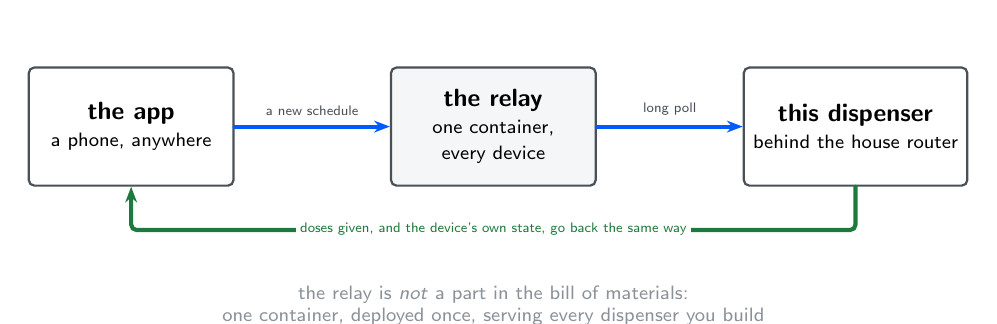
\begin{tikzpicture}
  \node[modbox, minimum width=26mm, minimum height=15mm] (app) at (-4.6,0)
       {\textbf{the app}\\[-0.3ex]{\scriptsize a phone, anywhere}};
  \node[modbox, minimum width=26mm, minimum height=15mm, fill=shade] (rel) at (0,0)
       {\textbf{the relay}\\[-0.3ex]{\scriptsize one container,}\\[-0.4ex]{\scriptsize every device}};
  \node[modbox, minimum width=26mm, minimum height=15mm] (dev) at (4.6,0)
       {\textbf{this dispenser}\\[-0.3ex]{\scriptsize behind the house router}};

  \draw[wire, i2cc, -{Stealth[length=2mm]}] (app.east) -- (rel.west)
       node[midway, above, font=\sffamily\tiny, text=ink70] {a new schedule};
  \draw[wire, i2cc, -{Stealth[length=2mm]}] (rel.east) -- (dev.west)
       node[midway, above, font=\sffamily\tiny, text=ink70] {long poll};
  \draw[wire, okgreen, -{Stealth[length=2mm]}]
       (dev.south) -- ++(0,-0.55) -- ($(app.south)+(0,-0.55)$) -- (app.south);
  \node[font=\sffamily\tiny, text=okgreen, fill=white, inner sep=1.5pt] at (0,-1.3)
       {doses given, and the device's own state, go back the same way};

  \node[font=\sffamily\scriptsize, text=ink40, anchor=north, align=center] at (0,-1.9)
       {the relay is \emph{not} a part in the bill of materials:\\
        one container, deployed once, serving every dispenser you build};
\end{tikzpicture}
\end{center}

\noindent See \code{../cloud\_relay/README.md}. Then name it here:

\begin{shell}
curl -X POST http://localhost/api/cloud \
     -H 'Content-Type: application/json' \
     -d '{"relayUrl":"https://snapcare-relay.fly.dev"}'
\end{shell}

\noindent or type it into the device's own console, or set
\code{SNAPCARE\_RELAY\_URL} in the systemd unit if you are building more than
one.

\begin{provebox}
\provetitle
\begin{shell}
curl -s http://localhost/api/status     # the "cloud" object
\end{shell}
\code{state} should reach \code{connected} within a few seconds, with
\code{lastError} empty and \code{reportedRev} at 1 or more \textemdash{} that
last one is the device having published its own state, which is what creates its
mailbox.

\vspace{1ex}
Then prove the direction that matters, from the relay's demo app: open
\code{https://<your relay>/lab}, pair with this device's code, and send it a
schedule. It should appear in \code{payload} here within a second or two.
\end{provebox}

\vspace{1mm}
\noindent\textbf{\sffamily If it does not:}

\begin{center}
\small
\begin{tabular}{@{}l >{\raggedright\arraybackslash}p{100mm}@{}}
\toprule
\hdr{\code{state}} & \hdr{What it means} \\
\midrule
\code{unpaired} & No relay URL. The POST above did not take, or was sent to the wrong host \\
\code{unsupported} & \code{python3-cryptography} is missing. \code{sudo apt install python3-cryptography} \\
\code{retrying} & The relay is not answering. \code{lastError} says why \textemdash{} usually DNS or a firewall \\
\code{offline} & It was reachable and has not been for fifteen minutes \\
\code{off} & Switched off \textemdash{} \code{-{}-no-cloud}, or \code{SNAPCARE\_CLOUD=0} \\
\bottomrule
\end{tabular}
\end{center}

\begin{dangerbox}
\dangertitle{The test nobody does: unplug the internet, not the device}
Pull the router's WAN cable, leave the dispenser on its LAN, and check that a
scheduled dose still comes out on time. It must. A build that has just gained a
cloud feature is exactly when a dependency on it gets introduced by accident,
and the symptom is a machine that works perfectly in every test anyone runs at a
desk.
\end{dangerbox}

\clearpage

% ═══════════════════════════════════════════════════════════════════════════
\section{Stage 10 \textemdash{} the label}

The setup code is printed once and never changes. It is derived, not generated:
HMAC-SHA256 over the SoC serial in \code{/proc/cpuinfo}, so it survives a
reimage and differs per board. The pairing code on it comes from the same
derivation, so it is permanent in the same way.

\begin{shell}
sudo python3 -m snapcare_dispenser --show-qr      # scannable, in the terminal
\end{shell}

\noindent or print the proper one from \code{http://pilldispenser.local/label}.

\vspace{3mm}
\begin{center}
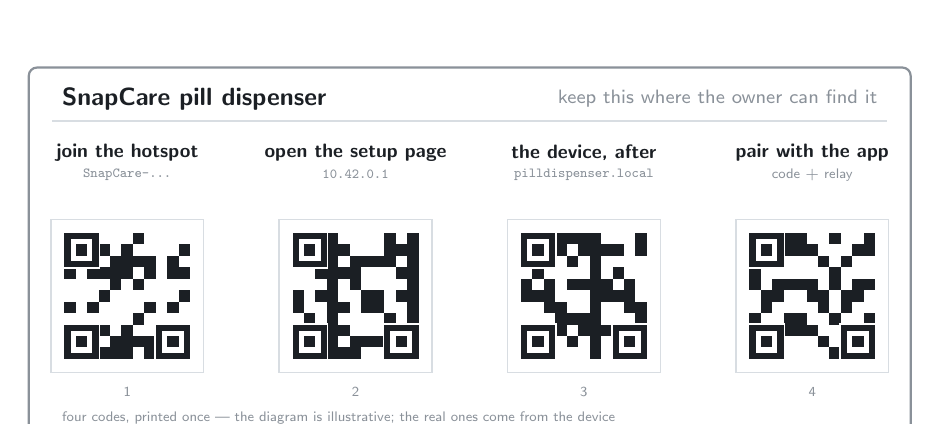
\begin{tikzpicture}
  \draw[ink40, line width=0.8pt, rounded corners=3pt, fill=white]
       (-5.6,-3.15) rectangle (5.6,1.5);
  \node[font=\sffamily\bfseries\small, text=ink, anchor=west] at (-5.3,1.1)
       {SnapCare pill dispenser};
  \node[font=\sffamily\scriptsize, text=ink40, anchor=east] at (5.3,1.1)
       {keep this where the owner can find it};
  \draw[ink15, line width=0.5pt] (-5.3,0.82) -- (5.3,0.82);

  \foreach \i/\ttl/\sub/\seed in {%
      0/{join the hotspot}/{\code{SnapCare-\ldots}}/2,
      1/{open the setup page}/{\code{10.42.0.1}}/3,
      2/{the device, after}/{\code{pilldispenser.local}}/5,
      3/{pair with the app}/{code $+$ relay}/7}{
    \pgfmathsetmacro{\x}{-4.35+\i*2.9}
    \begin{scope}[shift={(\x-0.85,-2.25)}]
      \draw[ink15, line width=0.5pt] (-0.12,-0.12) rectangle (1.82,1.82);
      \begin{scope}[shift={(0.05,0.05)}]\fakeqr{1.6}{\seed}\end{scope}
    \end{scope}
    \node[font=\sffamily\scriptsize\bfseries, text=ink] at (\x,0.42) {\ttl};
    \node[font=\sffamily\tiny, text=ink40] at (\x,0.14) {\sub};
    \node[font=\sffamily\tiny, text=ink40] at (\x,-2.62) {\the\numexpr\i+1\relax};
  }
  \node[font=\sffamily\tiny, text=ink40, anchor=west] at (-5.3,-2.95)
       {four codes, printed once \textemdash{} the diagram is illustrative; the real ones come from the device};
\end{tikzpicture}
\end{center}

\begin{dangerbox}
\dangertitle{The pairing code is a credential}
Anyone who can read it can send this device a schedule, in the same way anyone
who can read the WiFi password can join the hotspot. Put the label where the
owner can find it and a visitor cannot \textemdash{} inside a battery door, or
on the underside.
\end{dangerbox}

\begin{warnbox}
\warntitle{The one part of the label that is not permanent}
The pairing QR encodes \emph{your relay's address} alongside the code, because
that is what makes a phone camera able to open it. Move to a different relay and
that QR points at the old one. The code printed beside it in text still works
\textemdash{} it is derived from the board, not from the relay \textemdash{} so
the fix is to reprint, not to re-pair. If you expect to move relays, print the
label with no relay configured: the QR then carries the code alone, which the
app can read and a plain camera cannot.
\end{warnbox}

\clearpage

% ═══════════════════════════════════════════════════════════════════════════
\section{The whole pin map, in one place}

\begin{center}
\small
\begin{tabular}{@{}c l >{\raggedright}p{25mm} >{\raggedright}p{26mm} >{\raggedright\arraybackslash}p{52mm}@{}}
\toprule
& \hdr{Signal} & \hdr{GPIO (BCM)} & \hdr{Header pin} & \hdr{Notes} \\
\midrule
\swatch{servo} & Servo tray 1 & 17 & 11 & signal only \textemdash{} \textbf{not} power \\
\swatch{servo} & Servo tray 2 & 27 & 13 & \\
\swatch{servo} & Servo tray 3 & 22 & 15 & \\
\swatch{resv}  & \emph{Servo trays 4--8} & \emph{5, 6, 13, 19, 26} & \emph{29, 31, 33, 35, 37} & reserved, unfitted \\
\swatch{ringc} & WS2812 ring data & 18 & 12 & through 330\ohm{} at the ring; must be 18/12/21/10 \\
\swatch{buzzc} & Piezo buzzer & 23 & 16 & through 100\ohm \\
\swatch{btnc}  & Confirm button & 24 & 18 & other leg to GND; internal pull-up \\
\swatch{i2cc}  & DS3231 SDA & 2 & 3 & the module's own pull-ups are enough \\
\swatch{i2cc}  & DS3231 SCL & 3 & 5 & \\
\swatch{p33}   & DS3231 VCC & \textemdash{} & 1 (3.3\,V) & not 5\,V \\
\swatch{gndc}  & Ground & \textemdash{} & 6, 9, 14, 20, 25, 30, 34, 39 & at least one to the servo supply GND \\
\bottomrule
\end{tabular}
\end{center}

\vspace{1mm}
\noindent Run \code{pinout} on the Pi for the full header. Everything above is
BCM numbering, which is what pigpio and RPi.GPIO both use.

% ═══════════════════════════════════════════════════════════════════════════
\section{Power budget}

Two supplies, and the split is the point.

\begin{center}
\small
\begin{tabular}{@{}l l l@{}}
\toprule
\hdr{Rail} & \hdr{Load} & \hdr{Draw} \\
\midrule
Pi supply (5\,V 2.5\,A) & Pi 3B with WiFi active & $\sim$0.4\,A idle, $\sim$1.2\,A peak \\
Servo supply (5\,V 2\,A$+$) & one SG90, moving & $\sim$0.2\,A typical, $\sim$0.7\,A stalled \\
Servo supply & WS2812 ring, 12\,px at brightness 60 & $\sim$0.15\,A ($\approx$0.7\,A at full white) \\
\bottomrule
\end{tabular}
\end{center}

\vspace{3mm}
\begin{center}
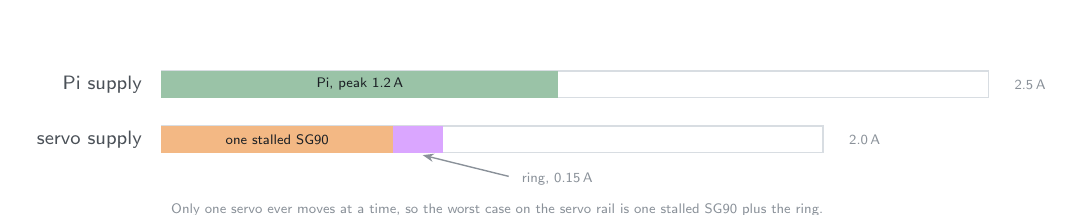
\begin{tikzpicture}[xscale=4.2, yscale=1]
  % --- Pi rail ---
  \node[font=\sffamily\scriptsize, text=ink70, anchor=east] at (-0.03,0.55) {Pi supply};
  \draw[ink15, line width=0.5pt] (0,0.38) rectangle (2.5,0.72);
  \fill[okgreen!45] (0,0.38) rectangle (1.2,0.72);
  \node[font=\sffamily\tiny, text=ink] at (0.6,0.55) {Pi, peak 1.2\,A};
  \node[font=\sffamily\tiny, text=ink40, anchor=west] at (2.55,0.55) {2.5\,A};

  % --- servo rail ---
  \node[font=\sffamily\scriptsize, text=ink70, anchor=east] at (-0.03,-0.15) {servo supply};
  \draw[ink15, line width=0.5pt] (0,-0.32) rectangle (2.0,0.02);
  \fill[servo!50] (0,-0.32) rectangle (0.7,0.02);
  \fill[ringc!35] (0.7,-0.32) rectangle (0.85,0.02);
  \node[font=\sffamily\tiny, text=ink] at (0.35,-0.15) {one stalled SG90};
  \node[font=\sffamily\tiny, text=ink40, anchor=west] at (2.05,-0.15) {2.0\,A};
  \draw[-{Stealth[length=1.4mm]}, ink40, line width=0.5pt] (1.05,-0.62) -- (0.79,-0.35);
  \node[font=\sffamily\tiny, text=ink40, anchor=west] at (1.06,-0.66) {ring, 0.15\,A};

  \node[font=\sffamily\tiny, text=ink40, anchor=west] at (0,-1.05)
       {Only one servo ever moves at a time, so the worst case on the servo rail
        is one stalled SG90 plus the ring.};
\end{tikzpicture}
\end{center}

\noindent Figures for the servo and the ring are the ones the firmware was
designed around; the Pi's are the usual published ranges. Meter your own rail if
you change the ring size or fit more than three trays.

\clearpage

% ═══════════════════════════════════════════════════════════════════════════
\section{Commissioning checklist}

Run this before the device goes anywhere near real medication.

\begin{shell}
curl -s http://localhost/api/status
\end{shell}

\vspace{1mm}
\begin{multicols}{2}
\begin{itemize}[leftmargin=*, label=\chk, itemsep=0.55ex, topsep=0.4ex]
\item \code{pigpio} backend, not \code{rpigpio} or \code{mock}
\item Clock trusted, source \code{rtc} or \code{ntp}
\item Ring \textbf{and} buzzer listed as fitted
\item Button backend \code{pigpio}
\item Three trays reported, matching the three that physically exist
\item Each \code{POST /api/drop} moves the hopper with the number you asked for
\item Servos silent and cool 5\,s after a drop
\item Pull the power mid-schedule, restore it: no second dose, and the log survives
\item Unplug the Pi's network, reboot: the DS3231 still vouches for the time
\item The printed label's QR joins the hotspot and opens the setup page
\item \textbf{Type the WiFi password wrong on purpose.} The setup network comes
      back within a few seconds and the page you re-open says the password was
      not accepted
\item Type it right: the ring stops being cyan and the device answers at
      \code{pilldispenser.local} from a phone back on the house WiFi
\item Change the router's password, reboot the device, wait: the setup hotspot
      appears on its own rather than the device sitting there unreachable
\item Power the router and the device off together and bring only the device back
      for a few minutes first. It raises its hotspot, then finds the router by
      itself once that returns \textemdash{} no hands
\end{itemize}

\vspace{1ex}
\noindent\textbf{\sffamily And if you did Stage 9:}
\begin{itemize}[leftmargin=*, label=\chk, itemsep=0.55ex, topsep=0.4ex]
\item \code{cloud.state} is \code{connected}, \code{lastError} empty
\item A schedule sent from the app appears in \code{payload} within a few seconds
\item A dose given here appears at the app end within a few seconds
\item \textbf{Cut the internet, keep the LAN: a scheduled dose still comes out on time}
\item Restore it: \code{state} returns to \code{connected} on its own, with
      nothing restarted
\item The doses given while it was offline arrive at the app afterwards
\item Send the same schedule revision twice: the second is ignored, not re-applied
\end{itemize}
\end{multicols}

\vspace{1mm}
\begin{notebox}
\textbf{\sffamily Three of these are worth doing properly rather than ticking.}

\vspace{1ex}
\textbf{The power cut.} A cut at 08:30 after the 08:00 dose is exactly the case
that dispenses twice without persisted state, and it is invisible in a demo.

\vspace{0.8ex}
\textbf{The internet cut.} Not the same test as unplugging the network, and it
is the one that catches a dependency on the relay introduced by accident
\textemdash{} because everything still passes at a desk with working internet.

\vspace{0.8ex}
\textbf{The repeated revision.} The relay refuses it, so the only way to see the
\emph{device's} own check is to test it here. That check is what stands between
a rolled-back relay and last month's prescription being applied as if it were
new.
\end{notebox}

\clearpage

% ═══════════════════════════════════════════════════════════════════════════
\section{When it does not work}

\begin{center}
\small
\begin{longtable}{@{}>{\raggedright}p{56mm} >{\raggedright\arraybackslash}p{92mm}@{}}
\toprule
\hdr{Symptom} & \hdr{Look at} \\
\midrule
\endhead
Servo twitches or ignores commands & Common ground. The Pi's GND and the servo supply GND must be joined \\
Servo hums between doses & You are on the \code{rpigpio} fallback \textemdash{} \code{sudo systemctl enable -{}-now pigpiod} \\
Servo buzzes at the end of a stroke & Being driven past its mechanical stop. Trim it in \code{SERVO\_TRIM} before it burns out \\
Pi reboots when a servo moves & Servos are on the Pi's 5\,V pin, or the rail has no bulk capacitor \\
Ring never lights, DMA error in the log & Data line is not on GPIO 18/12/21/10 \\
First pixel is the wrong colour & 330\ohm{} missing, or at the Pi end instead of the ring end. If it persists, the ring's 5\,V logic threshold ($0.7 \times V_{DD} = 3.5$\,V) is above the Pi's 3.3\,V output \textemdash{} shorten the lead, or drop the ring's supply to $\sim$4.5\,V \\
Ring flickers only when a servo moves & pigpio and the ring contending for PWM. Start pigpiod with \code{-t 0} to pin it to PCM \\
Buzzer makes a tone but not \emph{this} tone & It is an active buzzer with its own oscillator. Use a passive element \\
One press logs several doses & Debounce \textemdash{} check \code{journalctl} says the \code{pigpio} button backend, not \code{poll} \\
Tray stays shut, nothing dispenses & The clock is not trusted. \code{sudo hwclock -r}, check the coin cell, then \code{POST /api/clock} \\
Clock right at shutdown, wrong at boot & \code{fake-hwclock} is back, overwriting the RTC. The installer disables it \\
\code{pilldispenser.local} does not resolve & avahi, and the hostname. The web app's \code{DEFAULT\_HOST} is that exact string \\
Ring is cyan and stays cyan & The device is on its own setup hotspot waiting to be put on a network. Join \code{SnapCare-\ldots} and the page opens itself \\
Setup page says ``did not hand out an address'' & The password was right and DHCP was not. Usually a router that needs restarting, or a MAC filter \\
The setup hotspot keeps disappearing for half a minute & That is the unattended retry finding a saved network worth trying. It stops once one works; raise \code{HOTSPOT\_RETRY\_S} if it is in the way of a bench session \\
A schedule POST answers 421 & The \code{Host} header is not a name this device answers to. Use \code{pilldispenser.local} or the IP; \code{SNAPCARE\_EXTRA\_HOSTS} adds a router's own domain \\
Setup page never leaves ``waiting\ldots'' & The phone has not gone back to the house WiFi. Switch it over; the page follows. If the device's own network reappeared, the password was refused \\
A schedule is refused by tray number & That tray is not fitted. \code{INSTALLED\_TRAYS}, or \code{SNAPCARE\_TRAYS=8} \\
Cloud \code{state: unsupported} & \code{sudo apt install python3-cryptography}. Everything else still works meanwhile \\
Cloud \code{state: retrying}, DNS in \code{lastError} & The Pi has no working resolver. It joined the WiFi but got no DNS, or the router blocks it \\
Cloud connects, but no schedule ever arrives & The app is paired to a different code. Compare \code{cloud.deviceId} here with the one the app shows \textemdash{} they must match exactly \\
The app shows the device as never seen & Nothing has written to the mailbox. Check \code{reportedRev} here is 1 or more \\
A schedule sent from the app is refused & \code{cloud.lastError} says why, in the same words the LAN API would use. Usually a tray that is not fitted \\
Cloud fine, but doses take minutes to appear & \code{SNAPCARE\_CLOUD\_IDLE\_S} is set. That is the cheap mode working as asked \\
\bottomrule
\end{longtable}
\end{center}

\vspace{2mm}
\noindent\textbf{\sffamily Nothing here needs the hardware to reproduce the
\emph{logic} side of it:}

\begin{shell}
make            # the full suite, no board, no servos, no network
make run        # the whole firmware on a laptop, mock servos, port 8099
make -C .. demo # the same, plus a relay and the demo app on localhost:8088
\end{shell}

\noindent \code{make run} is the real firmware with the servo driver swapped for
one that records what it was told \textemdash{} the API, the scheduler, the web
console and the persistence all work, and nothing moves. \code{make demo} adds
the other end: a relay and a browser page that pairs with it, so the whole cloud
path can be exercised, including the failure cases, without a Raspberry Pi
anywhere.

\vfill
\begin{center}\footnotesize\color{ink40}\sffamily
This guide is generated from \code{docs/assembly-guide.tex} and follows
\code{ASSEMBLY.md}.\\
The pin map it describes lives in \code{snapcare\_dispenser/config.py}, which is
the source of truth.
\end{center}

\end{document}
